\chapter{Semi-supervised 3-D Constellation Model from Unknown Poses}
\label{chap/3dreg}

% intro 

\begin{figure}[ht]
\centering
\begin{subfigure}[b]{0.19\linewidth}
	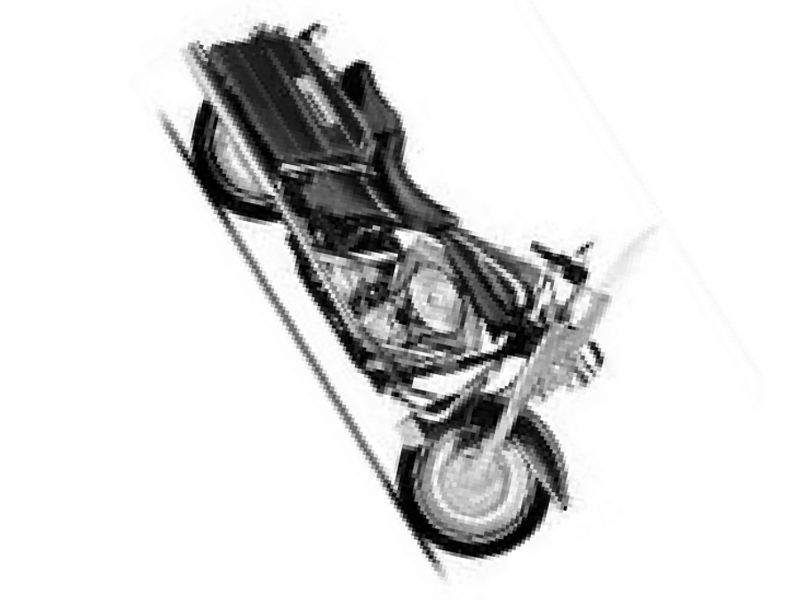
\includegraphics[width=\linewidth]{fig/3dreg/onebike_before2.png}
	\caption{Input instance}
	\label{fig:concept1}
\end{subfigure}
\begin{subfigure}[b]{0.19\linewidth}
	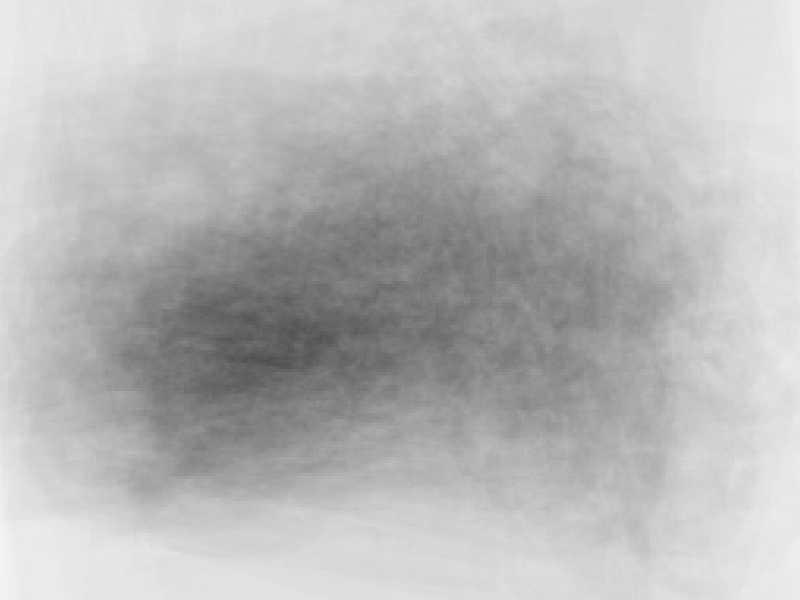
\includegraphics[width=\linewidth]{fig/3dreg/avgbike_before.png}
	\caption{Mean instance}
	\label{fig:concept2}
\end{subfigure}
\begin{subfigure}[b]{0.19\linewidth}
	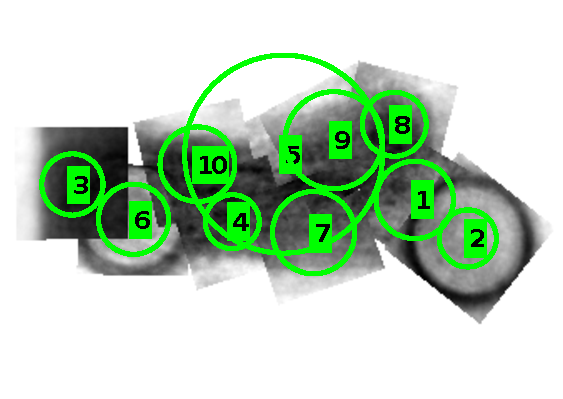
\includegraphics[width=\linewidth]{fig/3dreg/pictorial2.pdf}
	\caption{Constellation model}
	\label{fig:concept4}
\end{subfigure}
\begin{subfigure}[b]{0.19\linewidth}
	\label{fig:concept3}
	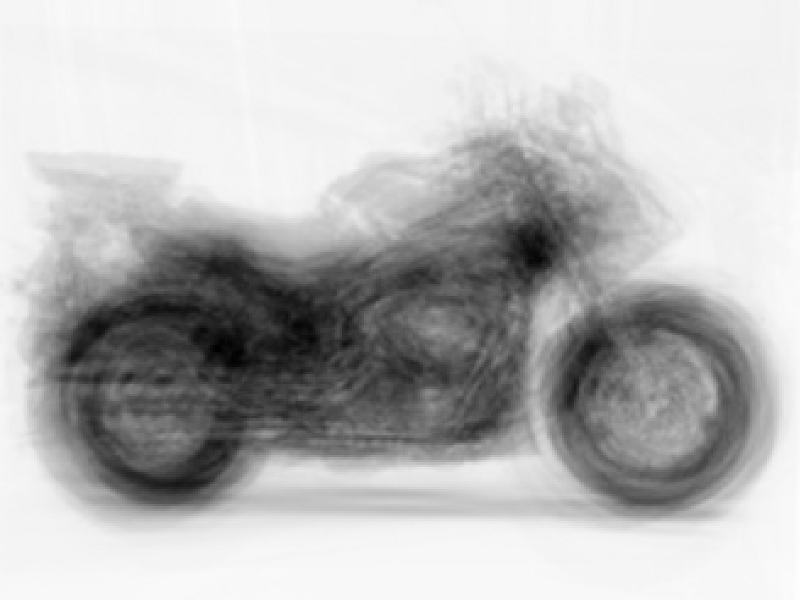
\includegraphics[width=\linewidth]{fig/3dreg/avgbike_after.png}
	\caption{Registered mean}
\end{subfigure}
\begin{subfigure}[b]{0.19\linewidth}
	\label{fig:concept5}
	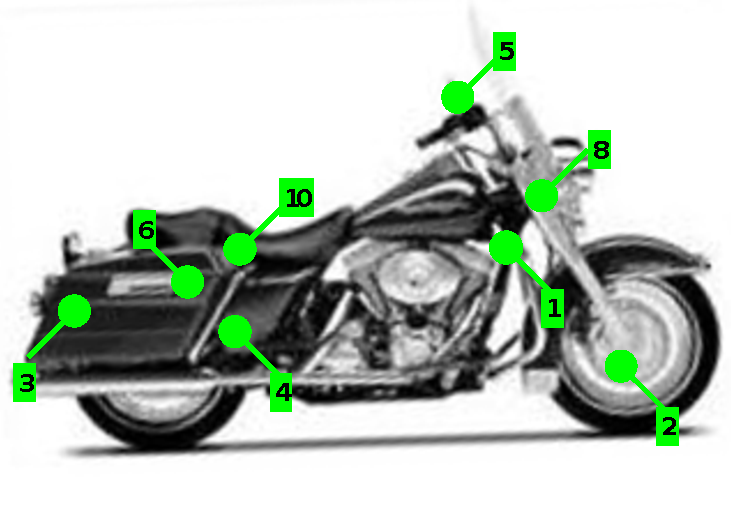
\includegraphics[width=\linewidth]{fig/3dreg/onebike_after3.pdf}
	\caption{Detected parts}
\end{subfigure}
\caption{(a) A training instance and (b) mean of input instances. (c) The learned constellation model, to which instances are \emph{simultaneously} registered during training. (d) The mean of registered input instances, weighted by their likelihoods, and (e) a registered instance with detected parts annotated.}
\label{fig:concept}
\end{figure}

\section{Introduction}
\label{sec:intro}

Part and vote-based methods have proved popular for object recognition tasks, overcoming the limitations of methods such as bag-of-words~\cite{Sivic2005, Fei-Fei2005} and topic models~\cite{Fergus2005}, by enforcing structural coherence within object classes. However, existing methods require pose information for learning---training data have to be aligned to a common reference frame \emph{a priori}---since modelling pose dramatically increases the dimensionality of the parameter space and hence inference complexity. This requirement precludes the use of internet-scale training datasets, \eg ImageNet~\cite{Deng2009} and Tiny Image Dataset~\cite{Torralba2008}, which are not generally annotated.

% Traditional computer vision tasks are usually approached by learning low level statistics on local, appearance based features, \eg bag of words~\cite{Sivic2005, Fei-Fei2005} and topic models~\cite{Fergus2005}, bypassing the high level structural information. These methods become less reliable in more challenging tasks, such as 3D shape recognition, when objects' textures are absent or weak in discriminative power. Making use of the spatial relationships among local features, part based model emerges as an effective solution for learning the geometric structure of an object class. Nevertheless, existing part based models require \emph{a priori pose information} for learning the structure of an object class---training data have to be registered to a common reference frame, involving extra manual processing when the poses of training or testing data are unknown. 

% Large scale image collections, such as Internet search engines or photo sharing services, have recently inspired various applications that utilize vast amounts of crowdsourced training data~\cite{Li2009, Simon2007}. However, processing these data is not trivial because the images are mostly unprocessed with varying poses and qualities, manual rectification is often required before passing the training data to learning algorithms. 

We address this issue with a framework, outlined in figure \ref{fig:concept}, for learning a shape, appearance and \emph{pose} (SAP) constellation model: training instances with various \emph{unknown} poses are used to learn a constellation model, as well as registrations for the instances. We therefore enable the use of training data without pose information for weakly-supervised learning of such models, and additionally provide a means of estimating the pose of both training and test instances. The technical contributions are two-fold: to present a generative probabilistic model which includes instance pose as a variable, and an optimization framework capable of solving the resulting, difficult inference problems.

% another unnecessary paragraph for lazy reviewers, I am thinking about removing this.
%The rest of this paper is organized as follows: The next section gives a brief literature review of related models and algorithms. The design and optimization of the proposed approach are detailed in section \ref{sec:framework}. We present the evaluation experiments in section \ref{sec:experiments} and conclude the paper in section \ref{sec:conclusions}.  

\subsection{Related Work}
\label{sec:relatedwork}

%%%%%%%%%%%%%%%%%%%%%%%%%%%%%%%%%%%%%%%%%%%%%%%%%%%%%%%%%%%%%%%%%%%%%%%%%%%%%%%%%%%%%%%%%%%%%%%%%
% fine
%%%%%%%%%%%%%%%%%%%%%%%%%%%%%%%%%%%%%%%%%%%%%%%%%%%%%%%%%%%%%%%%%%%%%%%%%%%%%%%%%%%%%%%%%%%%%%%%%
Local, feature-based methods are widely used in object recognition tasks, thanks to their robustness to occlusion. While some approaches, such as bag-of-words \cite{Sivic2005, Fei-Fei2005} and topic models \cite{Fergus2005}, use only the categorical distribution of appearance features, others such as constellation (or part-based) and vote-based models utilize the structural coherence of an object class, at a cost of lower flexibility to pose changes.

Part-based models were first articulated by Fischler and Elschlager \cite{Fischler1973} and Marr \cite{Marr1982} as a collection of templates or shape primitives. While early implementations were class-specific, \eg faces \cite{Yuille1989}, they have become more general: Burl \etal~\cite{Burl1998} trained a constellation model from hand-picked parts represented as Gaussian distributions. Weber \etal \cite{Weber2000} improved the former approach by using an interest point detector \cite{Kadir2001} to learn feature words and approximating the feature-part assignment marginal. Fergus \etal \cite{Fergus2007} introduced scale-invariance to the model and learnt shape and appearance models jointly. 
The constellation model has since been applied to 3D shape recognition~\cite{MuktaPrasad2011} also.

%<<<<<<< HEAD
%%%%%%%%%%%%%%%%%%%%%%%%%%%%%%%%%%%%%%%%%%%%%%%%%%%%%%%%%%%%%%%%%%%%%%%%%%%%%%%%%%%%%%%%%%%%%%%%%
% What to do? learn relative poses! But how?
%%%%%%%%%%%%%%%%%%%%%%%%%%%%%%%%%%%%%%%%%%%%%%%%%%%%%%%%%%%%%%%%%%%%%%%%%%%%%%%%%%%%%%%%%%%%%%%%
%Although object poses have been partially approached in part-based models(translation and scale)~\cite{Fergus2007}, \emph{training} instances have to be registered in advance, which becomes a major limitation of part-based model. To learn a the shape of an object class without the poses of training data, it is necessary to estimate poses from matching local features. 
%Early solutions to this task include ICP~\cite{Besl1992} and RANSAC~\cite{Fischler1981}. However, they rely on parameter initialization, which suffer from the local minima. Recently, Learned-Miller proposed congealing~\cite{Learned-Miller2006} which is a data-driven method for registering an image collection. 

%%%%%%%%%%%%%%%%%%%%%%%%%%%%%%%%%%%%%%%%%%%%%%%%%%%%%%%%%%%%%%%%%%%%%%%%%%%%%%%%%%%%%%%%%%%%%%%%%
% Why not use vote-based methods?
%%%%%%%%%%%%%%%%%%%%%%%%%%%%%%%%%%%%%%%%%%%%%%%%%%%%%%%%%%%%%%%%%%%%%%%%%%%%%%%%%%%%%%%%%%%%%%%%%
%In this latter category are vote-based and constellation (or part-based) methods. Vote-based methods use each feature to cast a set of votes, computed from a non-parametric distribution, for the pose and class of an object, seeking modes in this vote space. By contrast, part-based methods tend to have parameterized distributions for the shape and appearance of object \emph{parts}, enforce a one-to-one mapping between parts and features, and require multiple matches to infer the pose of an object. They are also more probabilistic 
%On the other hand, vote-based methods are popular alternatives to constellations, which have been applied in image recognition~\cite{Shotton2008a, Leibe2008} and 3D shape recognition~\cite{Flitton2010,  Knopp2010, Pham2011, Barinova2012}. 
%Vote-based approaches also use the spatial relationship among local features, but in a different manner: 
%They share similarities with part-based models, yet they are also fundamentally different. 
%Both methods consider an object class as a collection of local features, with a consistent geometric structure among its exemplars. 
%Both methods consider an object class as a collection of local features, with their geometric structure described in the model. 
%In addition, a test object is recognized by finding the class model that gives the highest likelihood from the assigned parts / votes. 
%Votes are cast by non-parametric code words, while parts in constellation models are usually parametrized as probability distributions. In contrast to part-based models, vote-based methods do not always enforce one-to-one associations between features and code words, although there exist exceptions, \eg~\cite{Woodford2011}. Distribution of background features are usually ignored in vote-based methods, which require preprocessing such as background subtraction~\cite{Leibe2004} and interleaved segmentation~\cite{Leibe2008} for discarding background features. 
%=======
Vote-based methods, \eg the implicit shape model \cite{Leibe2008} and contour fragments \cite{Shotton2008a}, which differ from constellation models in that each feature vote consists of a complete object pose and class, the internal object representation tends to be non-parametric, and there is no model for background clutter, allow for much faster inference at test stage. They too have been applied to both image-based \cite{Leibe2008, Shotton2008} and 3D shape recognition \cite{Flitton2010,  Knopp2010, Pham2011, Barinova2010}.

Although these part and vote-based methods can be used to infer pose at test, they all require \emph{registered} training instances for learning. 
This registration can be estimated from matching local features in a pre-processing step, using ICP \cite{Pham2011}, RANSAC \cite{Moreels2007}, bunch graph matching \cite{Wiskott1997} and matrix factorization \cite{Arie-Nachimson2009}, but these require either good initializations or manual annotations for bootstrapping. Alternatively, Learned-Miller \cite{Learned-Miller2006} proposed a data-driven method for registering an image collection. However, we know of no methods which learn a shape and appearance model and infer pose of training instances \emph{jointly}.

% This file includes the "model" and "inference" sections. 

% The Model Section
% - The conceptual design of the pose-shape model, i.e. how a feature is generated from parts
% - Graphical model and the explanation of different variables 
% - Learning objective
% - Testing objectives (registration and recognition)
% - Appearance model
% - Shape model

% The inference Section
% - The MCEM alorithm: Why, What and How?
% - The Pose optimization - simplification using the delta-pose update

% I am thinking whether we should explicitly write the entire gaussian function out in the inference section
% It depends on whether we have space for showing the maximizating steps or not (They should be in the supplementary materials anyway)

\section{Framework}
\label{sec:framework}
The aims of our framework are two-fold:
Firstly, given a set of $\numinstance$ data instances (\eg images or point clouds) with a particular class label, \ie an object of that class exists \emph{somewhere} in the data, to learn a constellation model for that object class.
Secondly, given a data instance of unknown class, to estimate the class label and pose of the object in the data.
\begin{figure}[ht]
\centering
\begin{subfigure}[b]{0.33\linewidth}
	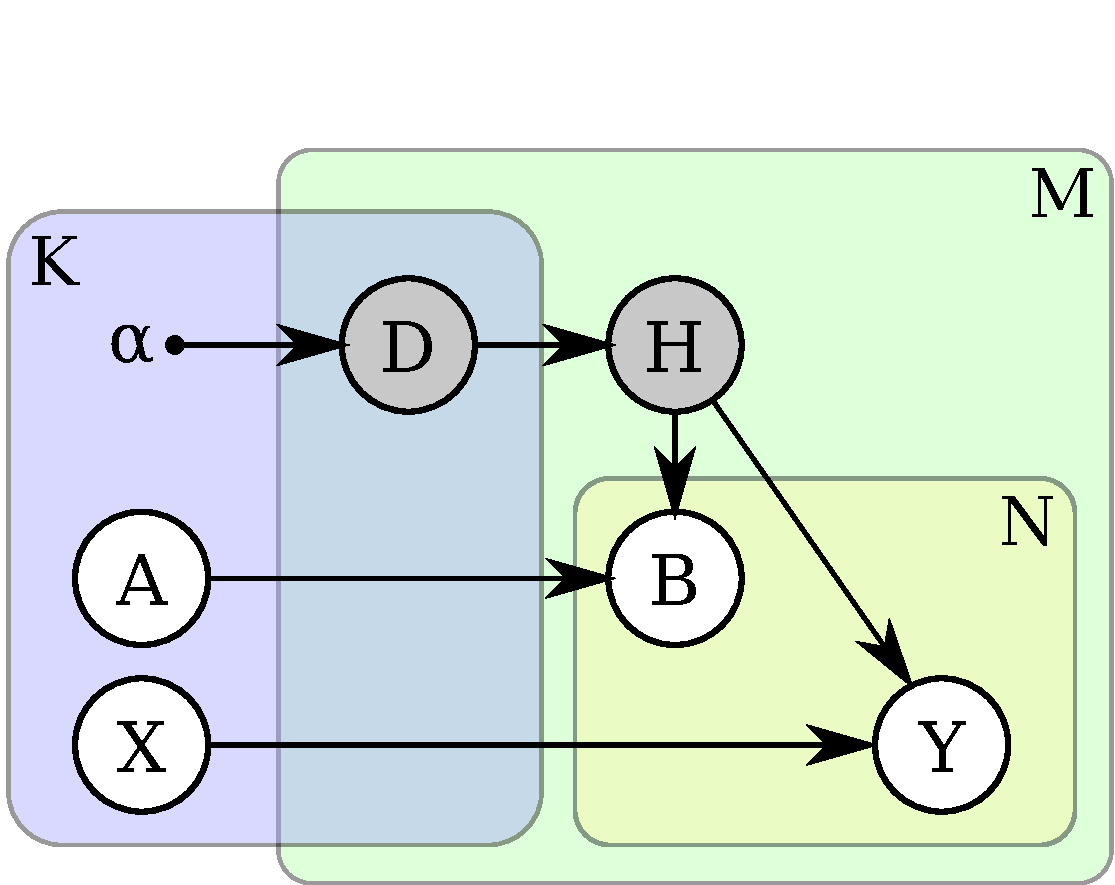
\includegraphics[width=\linewidth]{fig/3dreg/graphicalModelNoPose.pdf}
	\caption{Traditional constellation model}	
	\label{fig:graphicalModelNoPose}
\end{subfigure}
\begin{subfigure}[b]{0.33\linewidth}
	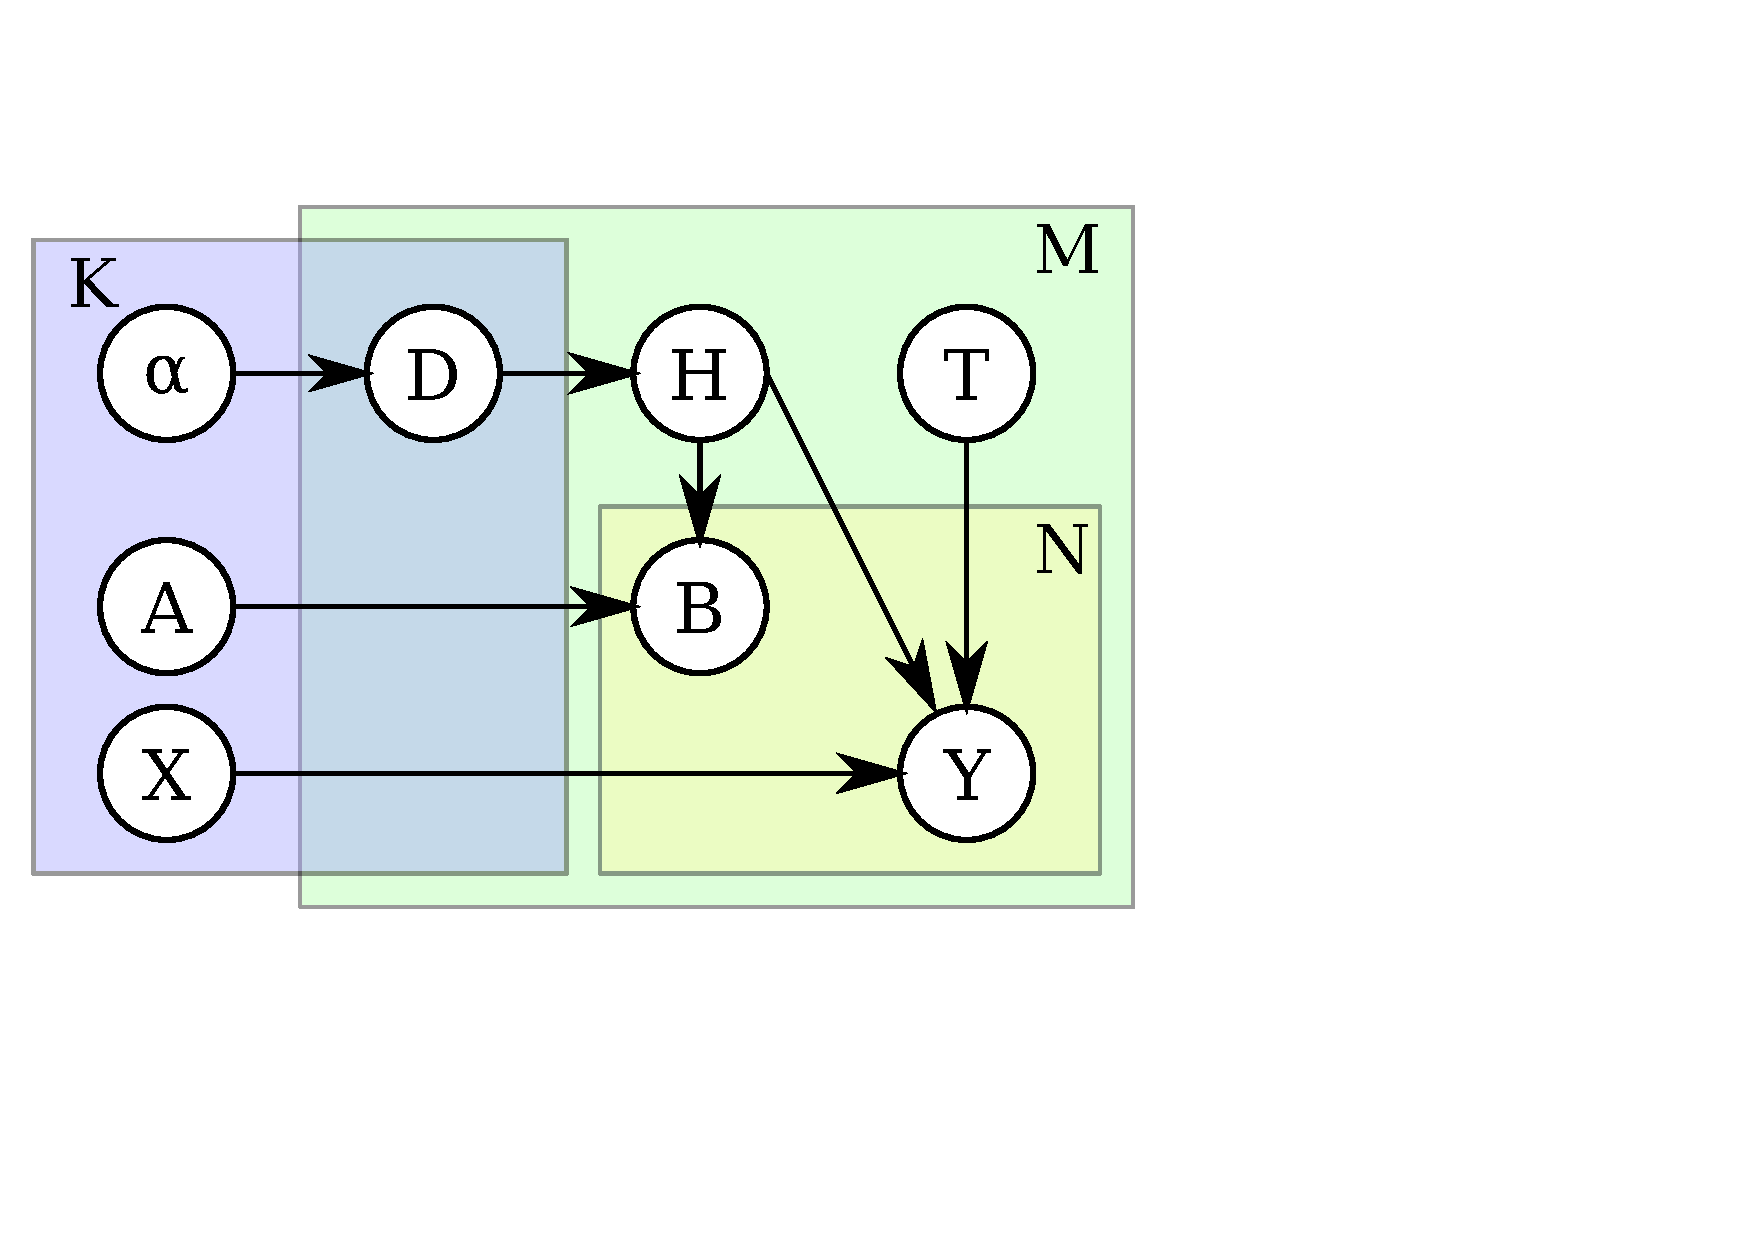
\includegraphics[width=\linewidth]{fig/3dreg/graphicalModelNoParticle.pdf}
	\caption{SAP model}	
	\label{fig:graphicalModelNoParticle}
\end{subfigure}
\begin{subfigure}[b]{0.33\linewidth}
	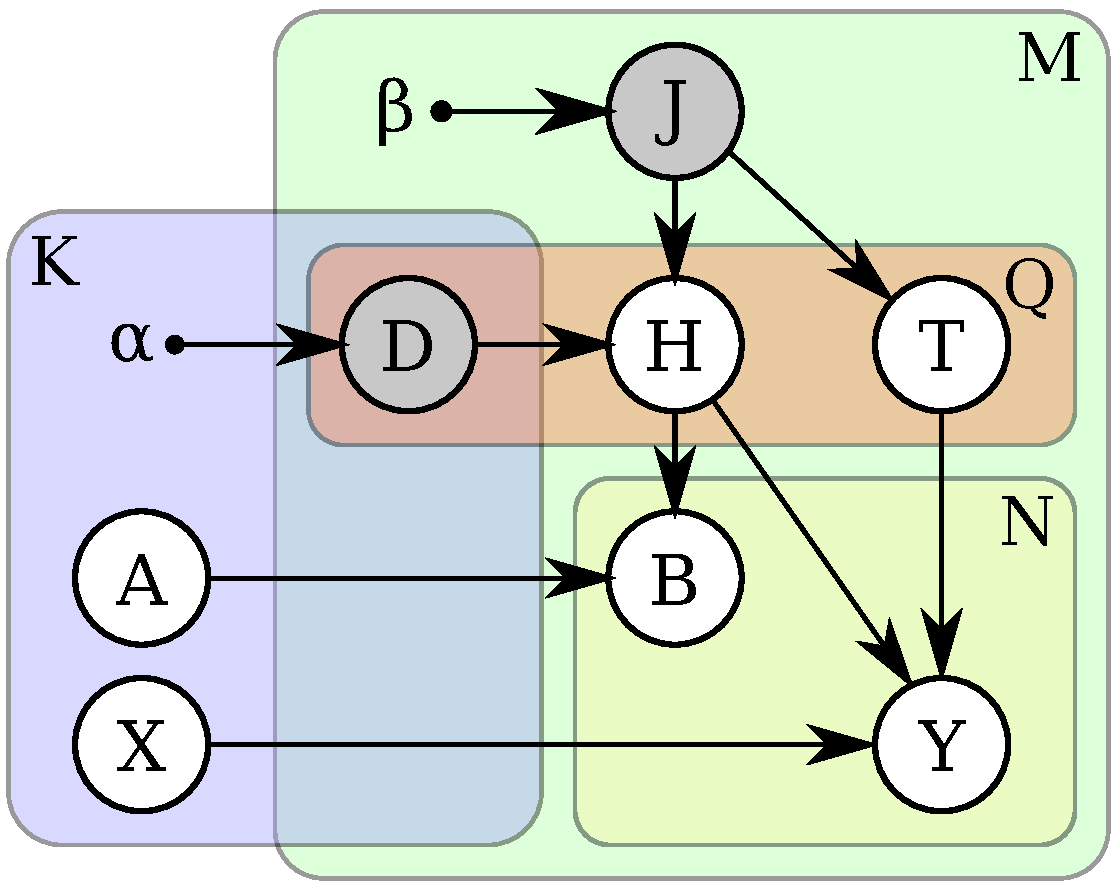
\includegraphics[width=\linewidth]{fig/3dreg/graphicalModelParticle.pdf}
	\caption{Approx. SAP with \emph{particles}}
	\label{fig:graphicalModelParticle}
\end{subfigure}
\caption{(a) Traditional constellation model. (b) The SAP model, to which we add a particle variable (c) to improve inference tractability. \emph{Grey}: latent variables.}
\label{fig:graphicalmodel}
\end{figure} 

\subsection{Model}
\label{sec:model}
A constellation model for a given object class is a generative model of the appearance and shape of that class, consisting of $\numpart$ object parts, each with an independent model (here, Gaussian with diagonal covariance) for appearance, $\partapp=\{\muapp,\sigmaapp\}$, and position, $\partshape=\{\mushape,\sigmashape\}$. Each part may or may not be seen in a given data instance, independently of other parts,\!\!\footnote{For simplicity, we assume independence of the presence of each part, in contrast to \cite{Fergus2007,Weber2000}, whose models are able to model correlations in part occlusion.} as indicated by the binary variable, $\seen$ ($=1$ if the part is seen). Following Fergus \etal \cite{Fergus2007}, we extract $\numfeat$ features\footnote{The number of extracted features, $\numfeat$, varies across instances; it is constant here for simplicity of exposition.} with pose $\featshape$ and appearance $\featapp$ from each data instance; the model assumes that each feature is generated either by a part from the object, or from an unknown background class (a single part with Gaussian appearance and pose distributions of $\{\muapp_0,\sigmaapp_0\}$ and $\{\mushape_0,\sigmashape_0\}$ respectively), according to an assignment, $\assign$. At most one feature can be assigned to a model part, whilst any number of features can be assigned to the background class, so that $\assign$, a $\numfeat\!\times\!(\numpart\!\!+\!\!1)$ binary indicator matrix, fulfils the constraints $\sum_{\anypart = 0}^{\numpart}\assignval_{\anyfeat\anypart}=1,\forall \anyfeat$ and $\sum_{\anyfeat = 1}^{\numfeat}\assignval_{\anyfeat\anypart}=\seen_\anypart,\forall \anypart>0$.\!\!\footnote{Since $\assign$ determines the $\seen$ values, the latter appear only for convenience, and are omitted where superfluous.} In addition, we novelly assume that the foreground object itself has a variable pose, $\pose$, completing the graphical model shown in figure \ref{fig:graphicalModelNoParticle}, which assumes there are $\numinstance$ training/test instances.

The appearance vectors $\muapp$ and $\featapp$ are parameterized according to the choice of feature descriptor, which is application dependent; we describe our choices in section \S\ref{sec:experiments}. The parameterizations of object and feature poses, which are also application dependent, have a large bearing on the tractability of the resulting inference problems, and are discussed in more detail in section \S\ref{sec:optimization}.

\paragraph{Notation}
Many of the random variables in the model are one of an independent set, indicated by the plates (boxes) in figure \ref{fig:graphicalmodel}. We denote the variable sets using the same letters in caligraphic font, while variables are indexed within these sets by subscript lowercase letters matching the uppercase letter indicating the number of elements in the set. For example, the set of part-feature assignments over all instances is $\setassign = \{\assign_{\anyinstance}\}_{\anyinstance=1}^\numinstance$. Set and subset indices are concatenated, \eg $\assignval_{\anyinstance\anyfeat\anypart}$.

\paragraph{Distributions}
We parameterize the various distributions in our model as follows:
\begin{align}
\prob(\seen_{\anypart}) = & ~\partprior_\anypart^{\seen_{\anypart}}\cdot(1-\partprior_\anypart)^{1-\seen_{\anypart}}, ~~~\partprior_\anypart\in[0, 1] \label{eqn:Ddist}\\
\prob(\assign|\setseen) = & \begin{cases} \frac{(\numfeat - \sum_{\anypart=1}^{\numpart}\seen_\anypart)!}{\numfeat!} & \mbox{if}~ \seen_\anypart = \sum_{\anyfeat=1}^{\numfeat}\assignval_{\anyfeat\anypart}, \forall\anypart\in\{1,..,\numpart\} \\ 0 & \mbox{otherwise} \end{cases}\label{eqn:HDdist}\\
\prob(\featapp|\setpartapp,\assign) = & \prod_{\anypart=0}^\numpart
\NormDist(\featapp; \muapp_\anypart, \sigmaapp_\anypart)^{\assignval_{\anyfeat\anypart}}
\label{eqn:appearance}\\
\prob(\featshape|\setpartshape,\assign,\pose) = & \prod_{\anypart=0}^\numpart
\left[\frac{\textstyle\exp(-\dist(\pose\comp\featshape, \mushape_\anypart; \sigmashape_\anypart)^2)}{\int_\mathbf{Z} \exp(-\dist(\mathbf{Z}, \mushape_\anypart; \sigmashape_\anypart)^2)}\right]^{\assignval_{\anyfeat\anypart}}\label{eqn:shape}
\end{align}
They are all relatively straightforward choices: a binomial prior over a binary variable, a uniform distribution over the valid assignments, and normal distributions around the appearance and position of the assigned part respectively, though the latter is in the non-Euclidean shape space, defined by the distance function, $\dist()$. 
% The $\comp$ operator represents the transformation of the LHS argument (a position) by the RHS argument (a pose).

\vspace{-0.5mm}
\subsection{Training}
During training we seek to maximize the posterior probability of the constellation model parameters, $\setpartapp$ and $\setpartshape$, with respect to the $\numinstance$ given instances:
\begin{equation}
\setpartapp,\setpartshape = \argmax_{\setpartapp,\,\setpartshape}
\prob(\setpartapp,\setpartshape)
\prod_{\anyinstance=1}^\numinstance 
\frac{\prob(\setfeatapp_\anyinstance,\setfeatshape_\anyinstance|\setpartapp,\setpartshape)}{\prob(\setfeatapp_\anyinstance,\setfeatshape_\anyinstance)}
 = \argmax_{\setpartapp,\,\setpartshape}
\prod_{\anyinstance=1}^\numinstance 
\prob(\setfeatapp_\anyinstance,\setfeatshape_\anyinstance|\setpartapp,\setpartshape),
\end{equation}
which, assuming $\prob(\setpartapp,\setpartshape)$ is uniform, is equivalent to maximizing their likelihood, since $\prob(\setfeatapp_\anyinstance,\setfeatshape_\anyinstance)$ is constant. Ordinarily this would be done whilst marginalizing over $\assign$ and $\pose$, which in this scenario are both latent variables, for each instance, thus:
\begin{equation}
\prob(\setfeatapp_\anyinstance,\setfeatshape_\anyinstance|\setpartapp,\setpartshape) = 
\sum_{\assign_\anyinstance \in \allassign}
\int_{\pose_\anyinstance}
\prob(\setfeatapp_\anyinstance,\setfeatshape_\anyinstance,\assign_\anyinstance,\pose_\anyinstance|\setpartapp,\setpartshape).
\label{eq:learningobjective}
\end{equation}
%usually using Expectation Maximization (EM).
However, given that the number of possible assignments, $|\allassign|$, is exponential in both $\numpart$ and $\numfeat$, whilst the instance pose, $\pose$, is a multi-dimensional, continuous variable in a non-Euclidean space, both the integrations are practically intractable. For this reason we introduce a particle-based approximation, described below.

\def\spfparticlem{\particle_{\anyinstance}\!\!=\!\!\anyparticle}
\def\spfparticle{\particle\!\!=\!\!\anyparticle}
\paragraph{Particle-based approximation}
We assume that the vast majority of the mass of the distribution in equation (\ref{eq:learningobjective}) occurs around the optimal configuration of pose and feature assignment for each instance, such that
\begin{equation}
\argmax_{\setpartapp,\,\setpartshape}
\prod_{\anyinstance=1}^\numinstance
\prob(\setfeatapp_\anyinstance,\setfeatshape_\anyinstance|\setpartapp,\setpartshape)
\approx 
\argmax_{\setpartapp,\,\setpartshape}
\prod_{\anyinstance=1}^\numinstance
\max_{\assign_\anyinstance,\,\pose_\anyinstance}
\prob(\setfeatapp_\anyinstance,\setfeatshape_\anyinstance,\assign_\anyinstance,\pose_\anyinstance|\setpartapp,\setpartshape).
\label{eq:approximatemaximumpose}
\end{equation}
This new objective function has many local maxima; a local optimization approach, initialized na\"{i}vely, will probably find a very poor solution. To overcome this we create $\numparticle$ pose \emph{particles} per instance, each with an associated feature assignment, and initialized randomly, to increase the chances of one finding the optimal solution. We then introduce a new latent variable, $\particle$, to our model: the index of the pose particle that represents the correct pose. This leads to the graphical model shown in figure \ref{fig:graphicalModelParticle}. Marginalizing over the $\numparticle$ possible values of $\particle$ per instance, given that $\prob(\pose_{\anyinstance\anyparticle}|\particle_{\anyinstance}\!\!=\!\!r)$ and $\prob(\assign_{\anyinstance\anyparticle}|\particle_{\anyinstance}\!\!=\!\!r)$ are delta distributions at $\anyparticle=r$, the final training objective function is therefore
\begin{equation}
\setpartapp,\setpartshape = \argmax_{\setpartapp,\,\setpartshape}
\prod_{\anyinstance=1}^\numinstance \sum_{\anyparticle = 1}^{\numparticle} 
\prob(\spfparticlem)
\max_{\assign_{\anyinstance\anyparticle},\,\pose_{\anyinstance\anyparticle}} \prob(\setfeatapp_\anyinstance,\setfeatshape_\anyinstance,\assign_{\anyinstance\anyparticle},\pose_{\anyinstance\anyparticle}|\setpartapp,\setpartshape),
\label{eq:particleapproximation}
\end{equation}
\begin{equation}
\prob(\setfeatapp,\setfeatshape,\assign,\pose|\setpartapp,\setpartshape) = 
\prod_{\anyfeat=1}^\numfeat
\prob(\featapp_{\anyfeat}|\setpartapp,\assign)
\prob(\featshape_{\anyfeat}|\setpartshape,\assign,\pose)
\sum_{\setseen}
\prob(\assign|\setseen)
\prod_{\anypart=1}^\numpart
\prob(\seen_{\anypart}).
\label{eqn:decompose}
\end{equation}
according to the decomposition specified by the model in figure \ref{fig:graphicalModelParticle}.
Note that the marginalization over $\setseen$ is trivial since equation (\ref{eqn:HDdist}) implies that, given $\assign$, only one value is possible. $\prob(\particle)$ is a categorical distribution:
$ \prob(\spfparticle) = \particleprior_\anyparticle$, where~~$ \sum_{\anyparticle=1}^\numparticle \particleprior_\anyparticle = 1.$ 
The particles can be seen as samples of the joint space of $\assign$ and $\pose$, making our approach similar to the Monte Carlo Expectation Maximization algorithm \cite{Levine2001, Wei1990}, which uses samples to approximate integrations over latent variables. However, we seek to maximize the likelihood of our particles, rather than draw them randomly from the distribution.

\subsection{Test}
At test stage we wish to estimate whether an object is present in the data, given the object class constellation model parameters, $\setpartapp$ and $\setpartshape$, and if so with what pose. The posterior probability of a given class being present would ideally be given by
\begin{equation}
\prob(\fg|\setfeatapp,\setfeatshape) = \frac{\prob(\fg)}{\prob(\setfeatapp,\setfeatshape)}\max_\pose \sum_{\assign \in \allassign}\prob(\setfeatapp,\setfeatshape,\assign,\pose|\setpartapp,\setpartshape),
\end{equation}
but, to avoid integrating over $\assign$, we use the same particle-based approximation as in training:
\begin{equation}
\prob(\fg|\setfeatapp,\setfeatshape) \approx \frac{\prob(\fg)}{\prob(\setfeatapp,\setfeatshape)} \sum_{\anyparticle=1}^\numparticle \prob(\spfparticle)
\max_{\pose_\anyparticle,\,\assign_\anyparticle} \prob(\setfeatapp,\setfeatshape,\assign_\anyparticle,\pose_\anyparticle|\setpartapp,\setpartshape),
\label{eqn:testobjective}
\end{equation}
which again decomposes according to equation (\ref{eqn:decompose}). The pose is then computed as the maximizing value of $\pose_\anyparticle$ for the most likely particle, \ie for which $\prob(\spfparticle)$ is largest.

This probability can then be used in binary or multi-class object classifiers by comparing the probabilities given for different object classes, including the background class (no object). The value $\prob(\setfeatapp,\setfeatshape)$ is constant across classes so can be ignored, while the a priori class distribution, $\prob(\fg)$, can be given or learned; here we assume it is uniform across classes.

\subsection{Optimization}
\label{sec:optimization}
Since both training and test objective functions, given by equations (\ref{eq:particleapproximation}) and (\ref{eqn:testobjective}) respectively, involve the latent $\particle$ variables, we maximize them using Expectation Maximization (EM), thus: 

\begin{algorithmic}[1]
	\STATE Initialize $\parameter^{(0)}$.
	\REPEAT
		\STATE \emph{E-step}: Evaluate the latent likelihood $\expect$ from $\parameter^{(t-1)}$.   
		\STATE \emph{M-step}: Maximize $\EMQ$ w.r.t. $\parameter^{(t)}$, in the following order: $\partprior^{(t)}$, $\particleprior^{(t)}$, $\assign^{(t)}$, $\partapp^{(t)}$, $\pose^{(t)}$ and $\partshape^{(t)}$.
	\UNTIL{convergence}
\end{algorithmic}
where $\parameter^{(t)} = \{\partprior^{(t)},\particleprior^{(t)},\assign^{(t)},\setpartapp^{(t)},\pose^{(t)},\setpartshape^{(t)}\}$ are the model parameters\footnote{$\setpartapp$ and $\setpartshape$ are udated during training, but not during test. That aside, the two optimizations are identical.} at iteration $t$, and
\begin{align}
\EMQ &= \sum_{\anyinstance=1}^\numinstance \sum_{\anyparticle = 1}^{\numparticle} 
\expect \log \left( \prob(\spfparticlem)\prob(\setfeatapp_\anyinstance,\setfeatshape_\anyinstance,\assign^{(t)}_{\anyinstance\anyparticle},\pose^{(t)}_{\anyinstance\anyparticle}|\setpartapp^{(t)},\setpartshape^{(t)}) \right), \\
\expect &= \frac{\prob(\spfparticlem)\prob(\setfeatapp_\anyinstance,\setfeatshape_\anyinstance,\assign^{(t-1)}_{\anyinstance\anyparticle},\pose^{(t-1)}_{\anyinstance\anyparticle}|\setpartapp^{(t-1)},\setpartshape^{(t-1)})}{\sum_{\anotherparticle = 1}^{\numparticle} \prob(\particle_{\anyinstance}\!\!=\!\!\anotherparticle)\prob(\setfeatapp_\anyinstance,\setfeatshape_\anyinstance,\assign^{(t-1)}_{\anyinstance\anotherparticle},\pose^{(t-1)}_{\anyinstance\anotherparticle}|\setpartapp^{(t-1)},\setpartshape^{(t-1)})}. 
\label{eq:auxiliary}
\end{align}
The updates for the M-step are obtained by setting the derivative of the auxiliary function $\EMQ$ w.r.t. each target parameter to zero. Since the parameters are interdependent, but optimized separately, this part of the algorithm effectively consists of an iteration of coordinate descent. The computations required for each step are described below.

\paragraph{Updating $\partprior$, $\particleprior$}  The update equations are
\newline
{\centering
\noindent\begin{minipage}{0.45\linewidth}
\begin{equation}
\partprior_{\anypart} = \frac{\sum_{\anyinstance=1}^\numinstance \sum_{\anyparticle = 1}^{\numparticle} \expect\seen_{\anyinstance\anyparticle\anypart}}{\sum_{\anyinstance=1}^\numinstance \sum_{\anyparticle = 1}^{\numparticle} \expect},
\end{equation}
\end{minipage}
\begin{minipage}{0.45\linewidth}
\begin{equation}
\particleprior_{\anyinstance\anyparticle} = 
\frac{\expect}{\sum_{\anyparticle = 1}^{\numparticle} \expect}.
\end{equation}
\end{minipage}
}

\paragraph{Updating $\assign$}
Taking negative logs of the terms in equation (\ref{eqn:decompose}) leads to a sum of costs to be minimized, all of which are linear in $\assign$, except for $-\log\prob(\assign|\setseen)$. However, if, as is generally the case, $\sum_{\anypart=1}^{\numpart}\seen_\anypart \ll \numfeat$, then this term is can be linearly approximated by $\sum_{\anypart=1}^{\numpart}\seen_\anypart\log\numfeat$, ($\seen_\anypart$ being a linear function of $\assign$). We compute the optimal $\assign$ for this approximate cost function in $\order\left((N\!+\!K)^3\right)$ time using a linear assignment solver such as the Hungarian method.

\paragraph{Updating $\setpartapp$}
The part appearances, $\partapp_\anypart$, are updated by computing a weighted mean and variance of the feature appearances, $\featapp_{\anyinstance\anyfeat}$, thus:
\begin{equation}
\wavg_k(x) = \frac{\sum_{\anyinstance=1}^\numinstance \sum_{\anyparticle = 1}^{\numparticle} \sum_{\anyfeat=1}^{\numfeat}\expect\assignval_{\anyinstance\anyfeat\anyparticle\anypart} \cdot x}{\sum_{\anyinstance=1}^\numinstance \sum_{\anyparticle = 1}^{\numparticle} \sum_{\anyfeat=1}^{\numfeat}\expect\assignval_{\anyinstance\anyfeat\anyparticle\anypart}}
\label{eq:weightedavg}
\end{equation}\vspace{-2mm}
\begin{equation}
\muapp_{\anypart}^{(t)} = \wavg_k(\featapp_{\anyinstance\anyfeat}), ~~~~ 
\sigmaapp_{\anypart}^{(t)} = \wavg_k((\featapp_{\anyinstance\anyfeat} - \muapp_{\anypart}^{(t)})(\featapp_{\anyinstance\anyfeat} - \muapp_{\anypart}^{(t)})^\trsp).
\label{eq:updatepartapp}
\end{equation}
% Since the weights depend on other part appearances, this does not compute the optimal $\setpartapp$, but is rather the first iteration of a reweighted-least-squares optimization. Nevertheless, only one iteration is used in each M-step, since the M-steps themselves are iterated.

\paragraph{Updating $\pose$}
The instance pose, $\pose$, can be parameterized in various ways, depending on the pose variations seen in the data. In this work we use two different parameterizations: The first is the direct similarity transform, 
\begin{equation}
\pose=\left[\begin{array}{cc}
s(\pose)\mathbf{R}(\pose) & \mathbf{t}(\pose)\\
\mathbf{0}^\trsp & 1\end{array}\right],
\label{eq:dsmatrix}
\end{equation}
where $s(\pose)\in\mathbb{R}^+$, $\mathbf{R}(\pose)\in SO(l,\mathbb{R})$, and $\mathbf{t}(\pose)\in\mathbb{R}^l$ are the scale, rotation, and translation components respectively, $l$ being the dimensionality of the space the data is in. In this case we parameterize the part/feature positions, $\partshape$ and $\featshape$, similarly, and use the SRT distance \cite{Pham2011} for $d()$ (in equation (\ref{eqn:shape})), with parameters $\sigmashape = \{\sigmashapes, \sigmashaper, \sigmashapet\}$, as this has the desirable properties of a closed form weighted mean and a constant Gaussian normalization factor. This not only eliminates scale bias \cite{Pham2011}, but also introduces feature orientation into the constellation model.

The second is the affine transform, represented by a matrix similar to that above, but whose first $l$ rows can take any real values. In this situation the part/feature positions are parameterized by translation only, and $d()$ is simply Euclidean distance.

The update equations for pose, and their derivations, are too extensive to detail here, so instead we sketch the update procedure. For the direct similarity transform, $\EMQ$ is differentiated w.r.t. each of the pose parameters in the order $\mathbf{t}(\pose)$, $\mathbf{R}(\pose)$, $s(\pose)$, and set to zero. For the first two components this yields a closed form update, while $s(\pose)$ is computed using Newton-Raphson. For the affine transform, setting the derivative to zero leads to a closed form update.

%Since the pose parameters are interdependent, this update is not optimal, but it does increase the model probability.
A degenerate case is where the pose scale component, $s(\pose)$, of any instance particle becomes zero. This issue is addressed by normalizing the weighted average pose scale to one at the end of each M-step. Since the SRT distance used in equation (\ref{eqn:shape}) is scale-invariant \cite{Pham2011}, this does not alter the model probability distribution. Such pose normalization changes the likelihood for the affine SAP model, however, the decrease in likelihood is approximately constant so it can be estimated without affecting the EM algorithm.

\paragraph{Updating $\setpartshape$}
The mean part positions, $\mushape_\anypart$, are updated according to \cite{Pham2011}, using the same weight as in equation (\ref{eq:weightedavg}). The bandwidth parameters are updated as follows:
\begin{align}
\sigmashapet_{\anypart}^{(t)} & = \wavg_k((\mathbf{t}(\featapp_{\anyinstance\anyfeat}) - \mathbf{t}(\mushape_{\anypart}^{(t)}))(\mathbf{t}(\featapp_{\anyinstance\anyfeat}) - \mathbf{t}(\mushape_{\anypart}^{(t)}))^\trsp),\label{eq:updatemeant}\\ 
\sigmashaper_{\anypart}^{(t)} & = \wavg_k((\mathbf{R}(\featapp_{\anyinstance\anyfeat}) - \mathbf{R}(\mushape_{\anypart}^{(t)}))(\mathbf{R}(\featapp_{\anyinstance\anyfeat}) - \mathbf{R}(\mushape_{\anypart}^{(t)}))^\trsp),\label{eq:updatedmeanr}\\
\sigmashapes_{\anypart}^{(t)} & = \wavg_k(\log^2(s(\featapp_{\anyinstance\anyfeat})/s(\mushape_{\anypart}^{(t)}))). \label{eq:updatemeans}
\end{align}
Since the affine poses cannot be uniquely factorized to SRT components, only the update steps for translation components, \ie $\mathbf{t}(\mushape_\anypart)$ and $\sigmashapet$, are performed for the affine pose SAP model. 

\paragraph{Initialization}
Initial parameters $\parameter^{(0)}$ for the EM algorithm are computed as follows: First, the particle poses $\pose^{(0)}$ for each instance are each assigned the inverse pose of an instance feature selected at random. Parameters $\partprior$ and $\particleprior$ are initialized uniformly as $1/2$ and $1/\numparticle$. $K$-means clustering is performed on the feature positions $\pose^{(0)}\featshape$, and initial parts $\{\partapp^{(0)}, \partshape^{(0)}\}$ are estimated from the $K$-means assignments. Finally, assignments $\assign^{(0)}$ are selected by maximizing the likelihood of the initial shape model.

\subsubsection{Particle considerations}
The computational cost of learning the model is linear in the number of particles, $\numparticle$, while there are diminishing returns to be had from increasing $\numparticle$, in terms of successful model convergence. The best number of particles is very much application and data dependent. In our experiments we found 5--10 particles were enough to give good results.

By allowing every instance to have multiple poses, equivalent sub-models can form within the model. To avoid this, after the first convergence of EM we select the instance with the highest likelihood and remove all but one of its particles (that with the highest likelihood), whose pose we then keep fixed, essentially defining the single \emph{canonical pose} of the class.

When the likelihood of particles heads to zero, or two or more particles converge on the same pose, updating them becomes computationally wasteful. To avoid this, those superfluous particles can either be removed, or their poses can be reinitialized at random. We use the latter, stochastic approach, to aid convergence to a good local optimum.

% TODO - 
% Restructure the section: divide it by datasets not applications (reg and rec)
% Since exact ground truth is not provided 

\section{Performance evaluation}
\label{sec:experiments}
We evaluate both registration performance (during both training and test) and recognition performance, on both 2D image data and 3D point cloud data.
% Experiments are performed to justify the versatility of our proposed shape-pose model under different types of input (2D images and 3D shapes) and applications (registration and recognition).  
%This section details the evaluations of the proposed approach and reports the experimental results.

\vspace{-2mm}
\subsection{Datasets}
% Maybe good to have a figure showing some sample data when we have enough space.
%The evaluation framework consists of two parts. 
%The first part evaluates the proposed model with respect to object recognition tasks. 
%The second part investigates the pose learning capability of the proposed approach. 
%Two types of data are used in the experiments to demonstrate the flexibility of the proposed model in different potential applications. 
% The model parameters, if not learned, are listed in table \ref{tab:parameters}. 
%\paragraph{Evaluation datasets} 
% 2D dataset, introduction
For the 2D evaluation we use the Caltech \emph{Bike} dataset~\cite{CaltechBike2001}, which contains 800 generic background images and 800 motorbike images with large inter-class appearance variations in cluttered backgrounds and moderately varying poses. Features are detected in each image over translation and scale, using the method described in \cite{Fergus2007}. Each feature position, $\featshape_{\anyinstance\anyfeat}$, is then completed by computing an $8$-quantized principal orientation from pixel gradients of the local patch. Appearance vectors, $\featapp_{\anyinstance\anyfeat}$, are computed by projecting the local patches into a compact 15-dimensional space using PCA.  

% 3D dataset, introduction
For the 3D evaluation we use the Toshiba CAD Model \emph{Point Cloud} dataset~\cite{ToshibaCAD2011}, which contains point clouds of 12 real objects acquired using multi-view stereo. Each object class contains 20 separate scans of a particular object, captured in a variety of poses. The dataset provides a set of features per point cloud, each with position in scale, rotation and translation, as well as a 31-dimensional descriptor, which we use for $\featshape_{\anyinstance\anyfeat}$ and $\featapp_{\anyinstance\anyfeat}$ respectively. The dataset additionally provides groundtruth pose for each object scan.
Similar to the \emph{Bike} dataset, the appearance descriptors are projected to a 10-dimensional subspace using PCA. More sophisticated features, \eg 3D shape context~\cite{Frome2004}, were tried in the experiments, but they showed similar performances with the default descriptor. The simpler default descriptor is therefore retained to demonstrate the effectiveness of the proposed model.

%\paragraph{Feature detection and representation} 
%Performance evaluations start with detecting local features $\featshape$ and their corresponding appearance information $\featapp$. For the \emph{Bike dataset}, translation and scale for each feature is detected using the method described in \cite{Fergus2007}. The pose a feature $\featshape$ is completed by estimating an $8$-quantized principal orientation based on its pixel gradients. Image patches are extracted and embedded to a compact $15$-dimensional space using PCA as $\featapp$.  
% For the \emph{Bike} dataset, features are located using the Kadir and Brady saliency detector~\cite{Kadir2001}. The SRT reference frames of detected interest points are completed by assigning an $8$-quantized principal orientation to each of them, according to the corresponding histogram of gradient. Rotated patches of the interest points are extracted from the images and resized to $15 \times 15$ pixels in size.
% The large $255$-dimensional space for appearance feature is embedded to a compact $15$-dimensional space using principal component analysis, for computation efficiency and noise reduction. 
%As point clouds are usually textureless, appearance features of the \emph{Point cloud} dataset are described by the local shape around the interest points. 
%The default interest points and descriptors of the \emph{Point cloud} dataset are used as off-the-shelf features.
\vspace{-2mm}
\subsection{Results: 2D images}
\paragraph{Recognition}
We use the evaluation framework of \cite{Fergus2007}, randomly dividing the \emph{Bike} dataset into two equal subsets, training on one half and testing on the other and vice versa and summing the results. Performance figures, shown in table \ref{tab:regresult2d}, are given by the ROC equal error rates for binary classification (so 50\% is the performance of a random classifier), testing against the background dataset. We test both the direct similarity and affine pose parameterizations against data with varying levels of both direct similarity and affine random transformations artificially applied to them, and compare with the results of Fergus \etal \cite{Fergus2007}.
% The \emph{Bike} dataset is split randomly into two separate subsets. 
%A two-fold cross-validation is performed by training the model on one subset and testing on the other. 
%Two-fold cross validation is performed by randomly dividing the \emph{Bike} dataset into two equal subsets. 
%In order to evaluate the model's pose learning ability, we introduced three different levels of synthetic extra transformations. 
%Hence, there are effectively seven datasets with different amounts of pose variations. 
\begin{table}
\centering
\begin{tabular}{|c|c|c|c|c|c|c|c|c|}
\hline
\multirow{2}{*}{\textbf{Method}} 	& \multirow{2}{*}{\textbf{$\numpart$,~$\numparticle$}} & \multirow{2}{*}{\textbf{No pose}}& \multicolumn{3}{|c|}{\textbf{Pose (similarity)}} 		& \multicolumn{3}{|c|}{\textbf{Pose (affine)}} \\
						& 	& & small & medium& large & small & medium & large \\
\hline
SAP (similarity) 		&	10, 5				& 95.500 & 94.625 & 93.250 & 92.250 & 92.750 & 79.000 & 71.250 \\
SAP (similarity)		&	6, 5				& 90.500 & 88.250 & 87.250 & 85.750 & 83.500 & 76.250 & 62.000 \\
\hline
SAP (affine) 			&	10, 5			& 95.125 & 92.125 & 83.125 & 75.750 & 91.000 & 75.500 & 71.000 \\
SAP (affine) 			&	6, 5				& 91.250 & 88.000 & 78.250 & 70.500 & 84.250 & 72.375 & 62.250 \\
\hline
Fergus \etal \cite{Fergus2007} 		& 6, -- & 95.125 & 87.000 & 60.000 & 52.000 & 86.375 & 59.250 & 52.000 \\
\hline
\end{tabular}

\caption{Recognition: ROC equal error rates for binary classification of the \emph{Bike} dataset.}
\label{tab:regresult2d}
\end{table}
\begin{figure}[ht]
\centering 
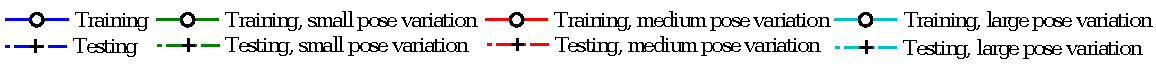
\includegraphics[width=0.80\linewidth]{fig/3dreg/reg2d_legend.pdf}
\begin{subfigure}[b]{0.23\linewidth}
	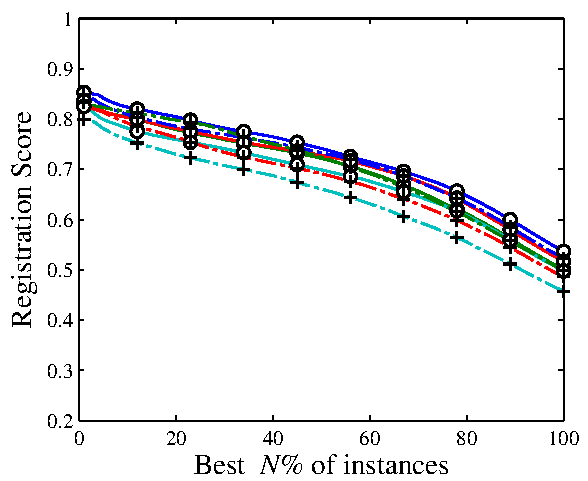
\includegraphics[width=\linewidth]{fig/3dreg/reg2d_simsim.pdf}
	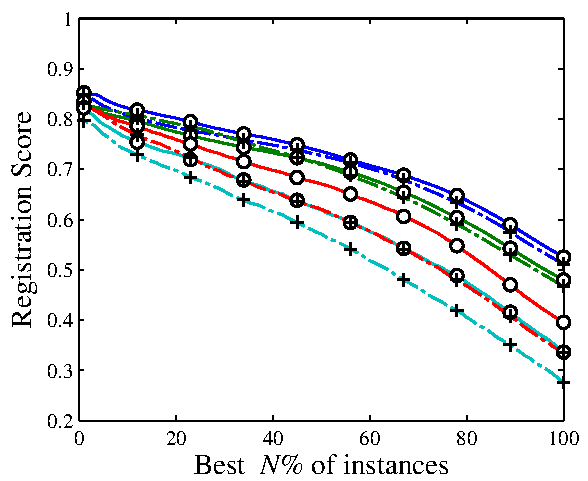
\includegraphics[width=\linewidth]{fig/3dreg/reg2d_simaff.pdf}
	\caption{SAP (pose model: similarity)}
\end{subfigure}
\begin{subfigure}[b]{0.23\linewidth}
	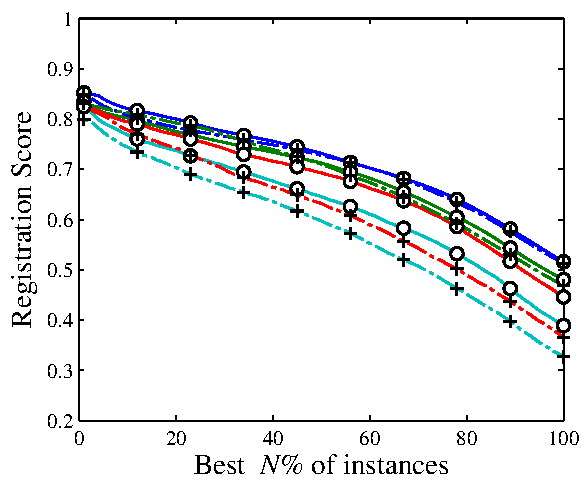
\includegraphics[width=\linewidth]{fig/3dreg/reg2d_affsim.pdf}
	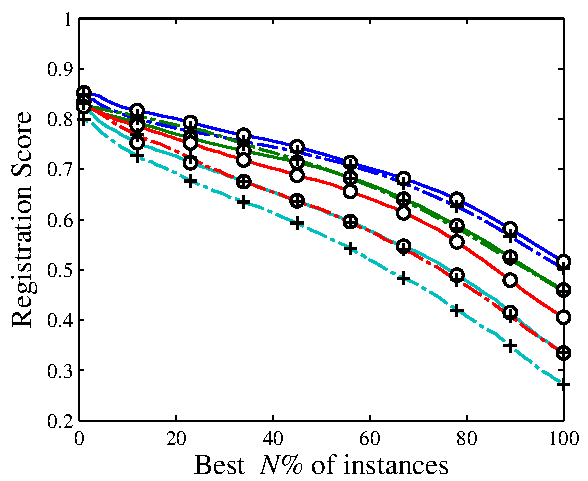
\includegraphics[width=\linewidth]{fig/3dreg/reg2d_affaff.pdf}
	\caption{SAP (pose model: affine)}
\end{subfigure}
\caption{Registration scores for the \emph{Bike} dataset. Two pose models, (a) similarity and (b) affine, are evaluated using data with synthetic (left) similarity and (right) affine poses.}
\label{fig:regresult2d}
\end{figure}

%Table \ref{tab:regresult2d} shows the recognition results using the proposed model and the work of Fergus \etal~\cite{Fergus2007}. 
Both approaches perform similarly when there is no or small pose variations, but the performance of~\cite{Fergus2007}, which does not model pose as a variable, drops rapidly as the pose variation level increases, with an accuracy similar to random classification under large pose variation.  By contrast, the SAP model with direct similarity pose maintains a high recognition rate under large direct similarity pose variations, while the affine model, for which feature rotation and scaling components are absent, performs slightly worse. Under affine transformations, the two types SAP model perform similarly, with a significant drop in performance under large pose variations; since the computed feature poses are not affine-invariant, the feature appearances are distorted by shearing, leading to a weaker appearance model.
%The SAP models experience a stable drop in accuracies when the level of pose variation increases. 
%The similarity pose SAP achieves a slightly better performance than its affine pose counterpart. 
%It is believed that the affine pose approach provides less useful information for object recognition, as the scaling and rotation components are absent in its shape model. 
% The more flexible affine transformations may also overfit the poses of some non-object testing instances, creating more false positives. 
%With a small shearing is added to the poses, 
%In addition, the SAP models reported lower accuracies in affine-transformed data, when a small shearing is added to the synthetic poses. Since the appearance features, \ie the rotated patches, are not affine invariant, they are irreversibly distorted by shearing so a weaker part appearance $\partapp$ is learned, affecting the accuracies.

\paragraph{Registration} 
%Since no ground truth poses are given in the original \emph{Bike} dataset, the registration results of the \emph{SAP} models are compared with hand-labeled pose information. 
%We create the registration dataset by selecting two hundred random object images from the \emph{Bike} dataset.
The registration score for the \emph{Bike} dataset is computed as follows: we manually annotated the front and rear wheel centres, $\refptfront$ and $\refptrear$, of 200 bikes. Similar to recognition, the dataset is divided into two halves for cross-validation. Reference points of both the training and testing instances are projected into the canonical pose, using the learned poses. The training data points are then used to learn two normal distributions, $\NormDist(\cdot;\mu_\mathrm{front},\Sigma_\mathrm{front})$ and $\NormDist(\cdot;\mu_\mathrm{rear},\Sigma_\mathrm{rear})$, modelling the wheel centre locations, plus a uniform outlier distribution, $\UniformDist(\backgroundreg)$, using the EM algorithm. A registration score in the range (0,1) is then computed for each training or test instance as
\begin{equation}
\mathcal{S}_\mathrm{reg} = \frac{\NormDist(\pose\refptfront; \mu_\mathrm{front},\Sigma_\mathrm{front}) + \NormDist(\pose\refptrear; \mu_\mathrm{rear},\Sigma_\mathrm{rear})}{\NormDist(\pose\refptfront; \mu_\mathrm{front},\Sigma_\mathrm{front}) + \NormDist(\pose\refptrear; \mu_\mathrm{rear},\Sigma_\mathrm{rear}) + 2\UniformDist(\backgroundreg)}.
\label{eq:reg2d_score}
\end{equation}
Figure \ref{fig:regresult2d} plots the registration scores under different levels of pose variation, which corroborate the recognition results in terms of relative performance. Comparable training and test scores indicate that the learned model transfers well to unseen data.
%The similarity-pose SAP model performs better than its affine-pose variant. Similar to the recognition experiment, it is mainly due to the lack of a full SRT shape model in the affine pose variant, and the geometric distortion of the appearance features. 

\vspace{-0mm}
\subsection{Results: 3D point clouds}

\paragraph{Recognition}
Following \cite{Pham2011}, we use a leave-one-out cross validation scheme to measure multi-class recognition accuracy on the \emph{Point Cloud} dataset. 
% One instance is taken out from the dataset each time as a test shape, while the remaining $19$ instances are used to train the object recognizer. 
Ten classes from the dataset are evaluated, thus 200 separate models are trained for the experiments.
% The optimal operating point, \ie decision threshold, is estimated from the training data when the false positive rate is smaller than $5\%$.

% {\centering
% \begin{minipage}{0.5\linewidth}
% \centering
% \label{fig:confusion_sap}
% 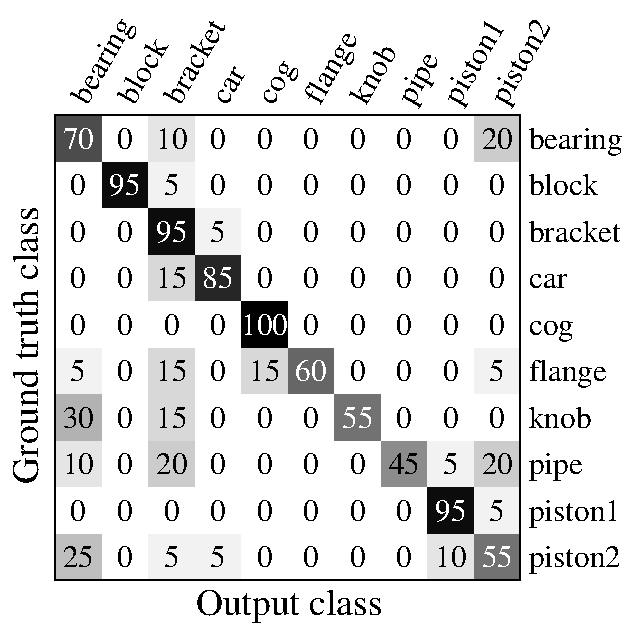
\includegraphics[width=0.5\linewidth]{fig/3dreg/confusion_sap.pdf}
% \vspace{2mm}
% \captionof{figure}{Conf. matrix of SAP model}
% \label{fig:recresult3d}
% \end{minipage}
% \hspace{-3mm}
% \begin{minipage}{0.5\linewidth}
% {\footnotesize
% \begin{tabular}{|c|c|}
% \hline
% \textbf{Approach} & \textbf{Average accuracy} \\ 
% \hline
% \emph{SAP} & 75.0 \\
% Min.-ent. Hough\remarka~\cite{Woodford2013} & 98.5 \\ 
% \hline
% \end{tabular} \\
% \remarka Supervised Hough voting-based method \\
% }
% \vspace{3mm}
% \captionof{table}{The average recognition accuracies.}
% \label{tab:recresult3d}
% \end{minipage}
% \vspace{2mm}
% }

% \begin{figure}[ht]
% \centering
% \hspace{-2mm}
% \subfigure[SAP]{
% 	\label{fig:confusion_sap}
% 	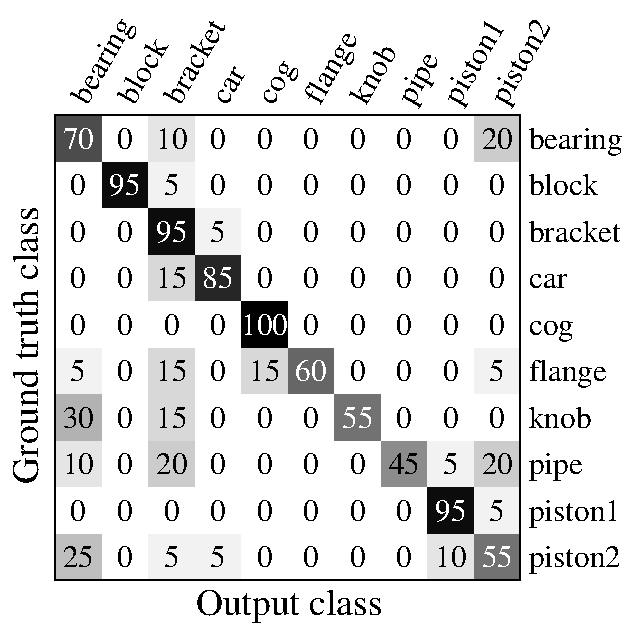
\includegraphics[width=0.2\linewidth]{fig/3dreg/confusion_sap.pdf}
%}
% \hspace{-4mm}
% \subfigure[Mean shift]{
% 	\label{fig:confusion_ms}
% 	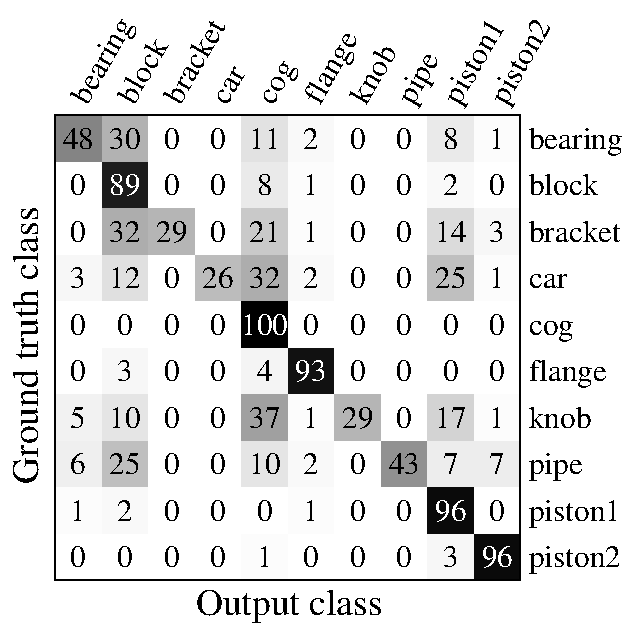
\includegraphics[width=0.2\linewidth]{fig/3dreg/confusion_meanshift.pdf}
% }
% \hspace{-4mm}
% \subfigure[Intrinsic H.]{
% 	\label{fig:confusion_int}
% 	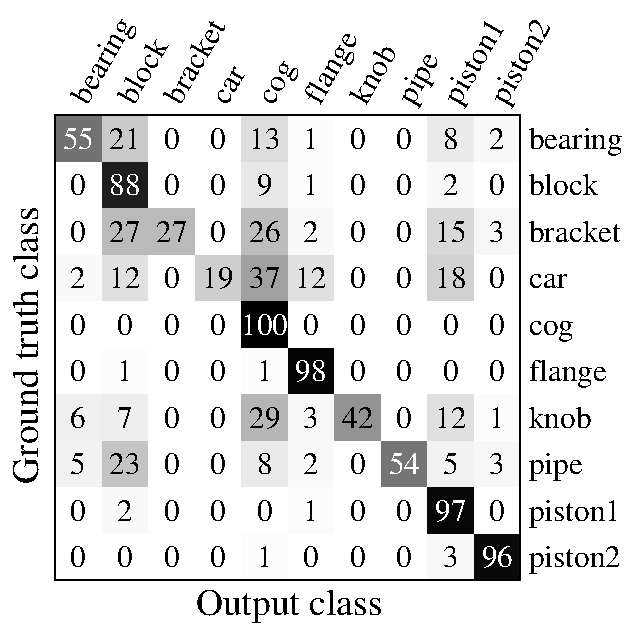
\includegraphics[width=0.2\linewidth]{fig/3dreg/confusion_intrinsic.pdf}
% }
% \hspace{-4mm}
% \subfigure[Min.-ent. H.]{
% 	\label{fig:confusion_minent}
% 	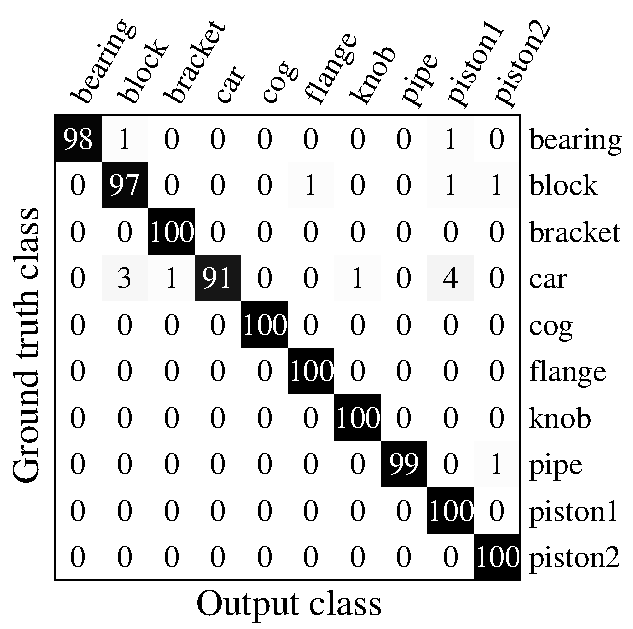
\includegraphics[width=0.2\linewidth]{fig/3dreg/confusion_minent.pdf}
% }
% \hspace{-4mm}
% \subfigure[BLK]{
% 	\label{fig:confusion_minent}
% 	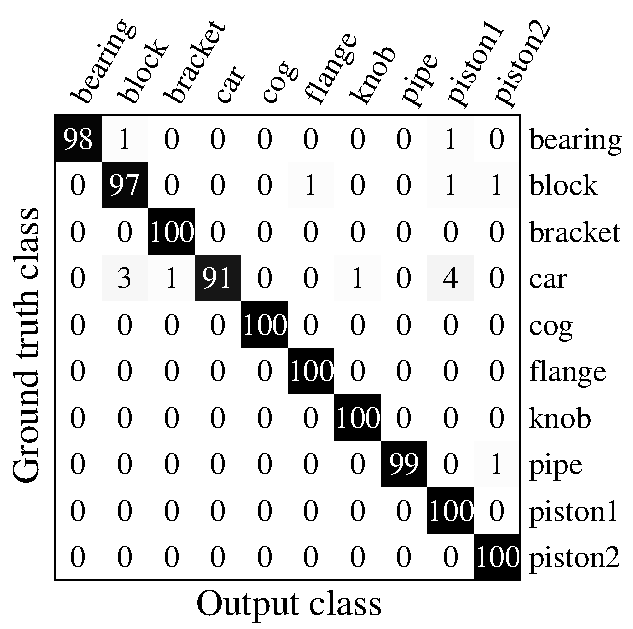
\includegraphics[width=0.2\linewidth]{fig/3dreg/confusion_minent.pdf}
%}
% \hspace{-4mm}
% \caption{The confusion matrices of (a) our approach, (b) Mean shift~\cite{Pham2011}, (c) Intrinsic Hough~\cite{Woodford2013}, (d) Minimum-entropy Hough~\cite{Woodford2013} and (e) BLK~\cite{Barinova2010}. Note that \emph{SAP} model is a binary object class recognizer, thus the rows of its confusion matrix are not sum to $100$.}
% \label{fig:recresult3d}
% \end{figure}


%\begin{table}
%\centering
%{\footnotesize
%\begin{tabular}{|c|c|c|c|c|c|}
%\hline
%\textbf{Approach} & \emph{SAP} & Mean shift~\cite{Pham2011} & Intrinsic H.~\cite{Woodford2013} & Min.-ent. H.~\cite{Woodford2013} & BLK~\cite{Barinova2010} \\ 
%\hline
%\textbf{Avg. acc. (\%)} & 75.0 & 64.9 & 67.6 & 98.5 & 98.1 \\ 
%\hline
%\end{tabular}
%}
%\caption{The average object recognition accuracies.}
%\label{tab:recresult3d}
%\end{table}

Figure \ref{fig:confusion_sap} shows the confusion matrix of the proposed SAP model, using the direct similarity pose parameterization.  
The weakly-supervised SAP model achieves satisfactory results of 75.5\% multi-class recognition accuracy, while the latest reported state-of-the-art accuracy, using groundtruth pose, is 98.5\%~\cite{Woodford2013}. %However, the combined multi-class classifier is biased towards some stronger classes, \eg \emph{bracket}, as shown in figure \ref{fig:confusion_sap}.

\paragraph{Registration} 
\label{sec:3dreg}
Registration of the \emph{Point Cloud} dataset is evaluated quantitatively using SRT distances~\cite{Pham2011} between pairs of instances. Given the groundtruth pose, $\pose_\mathrm{gt}$, of an instance, the learned pose relative to the groundtruth object coordinate frame is $\tilde{\pose} = \pose_\mathrm{gt}\pose^{-1}$. We use the registration criterion of~\cite{Pham2011}: A pair of instances is correctly registered when their $\tilde{\pose}$ are within 5\% in scale, $\pi$/12 in orientation and 10\% in relative translation.

\begin{figure}[ht]
	\centering
	\begin{subfigure}[b]{0.20\linewidth}
		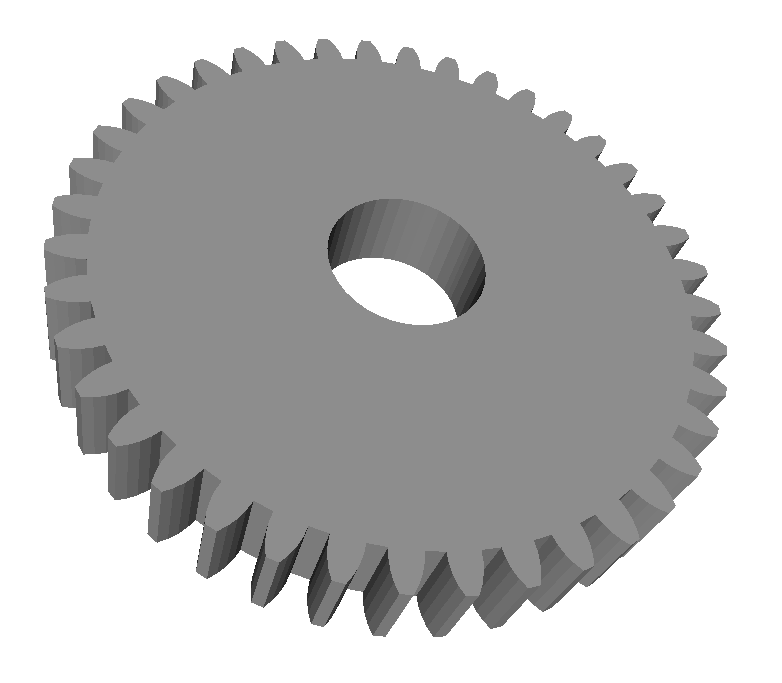
\includegraphics[width=\linewidth]{fig/3dreg/cog.png} \\
		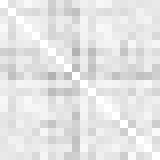
\includegraphics[width=\linewidth]{fig/3dreg/reg3Dtrain_cog.png} 
		\caption{Cog}
	\end{subfigure}
	\begin{subfigure}[b]{0.20\linewidth}
		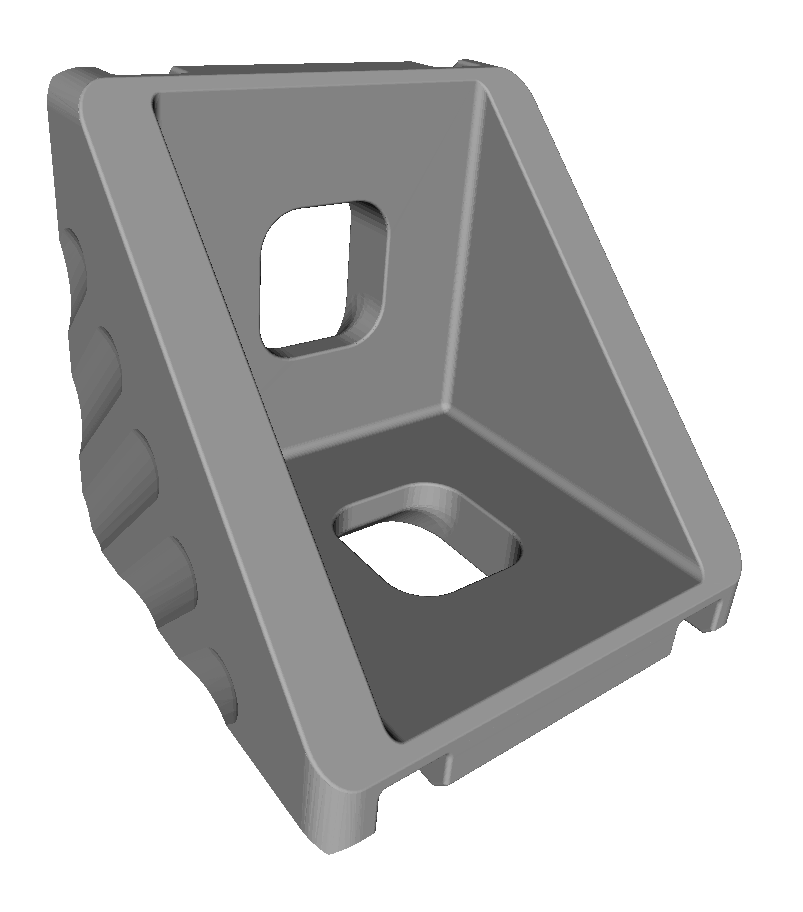
\includegraphics[width=\linewidth]{fig/3dreg/bracket.png} \\
		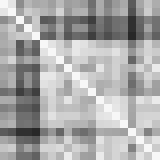
\includegraphics[width=\linewidth]{fig/3dreg/reg3Dtrain_bracket.png} 
		\caption{Bracket}
	\end{subfigure}
	\begin{subfigure}[b]{0.20\linewidth}
		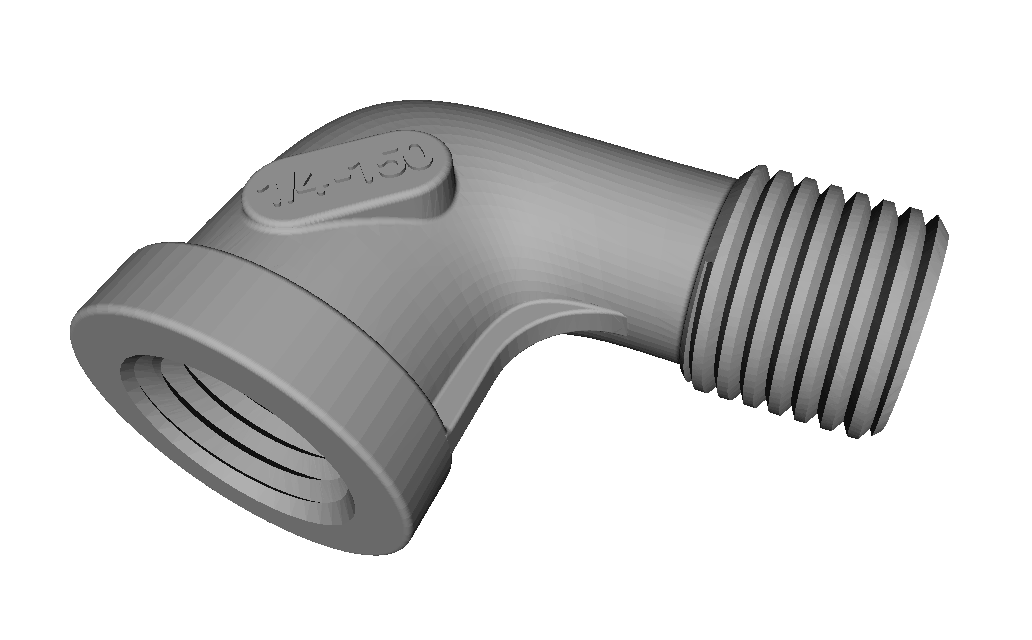
\includegraphics[width=\linewidth]{fig/3dreg/pipe.png} \\
		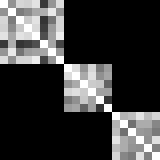
\includegraphics[width=\linewidth]{fig/3dreg/reg3Dtrain_pipe.png} 
		\caption{Pipe}
	\end{subfigure}
	\begin{subfigure}[b]{0.20\linewidth}
		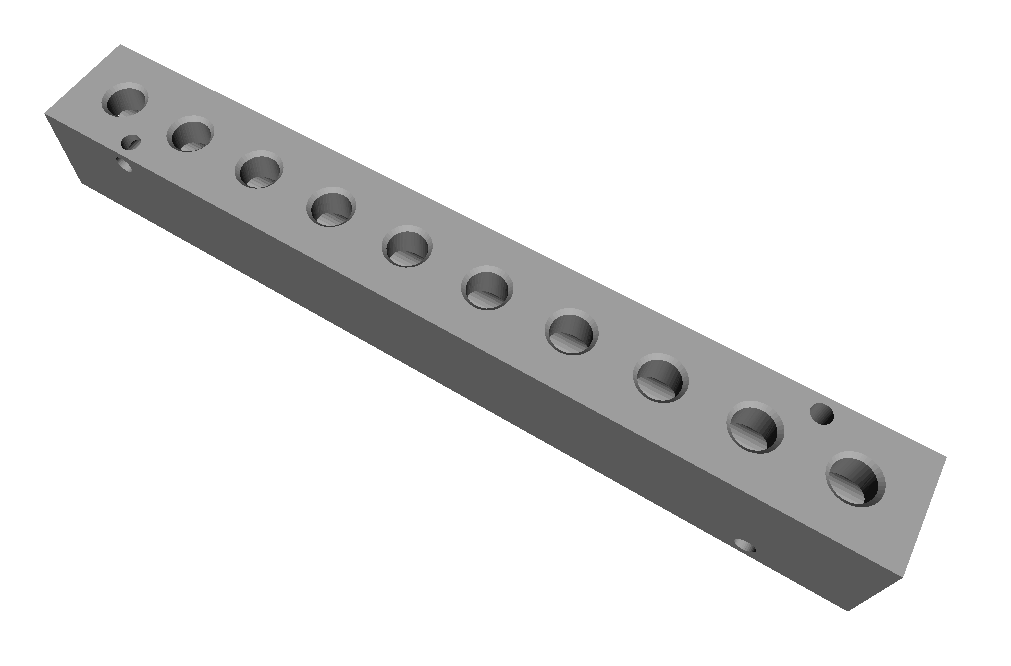
\includegraphics[width=\linewidth]{fig/3dreg/block.png} \\
		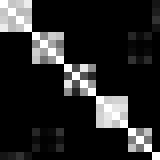
\includegraphics[width=\linewidth]{fig/3dreg/reg3Dtrain_block.png} 
		\caption{Block}
	\end{subfigure}
	\caption{Distance matrices, in $\exp(-\dist())$ where $\dist()$ is the SRT distance. Note that the bad resgistred classes, \eg \emph{block}, are clustered.}
	\label{fig:3dreg_srtmatrices}
\end{figure}

\begin{figure}[ht]
	\centering
	\begin{subfigure}[b]{0.20\linewidth}
		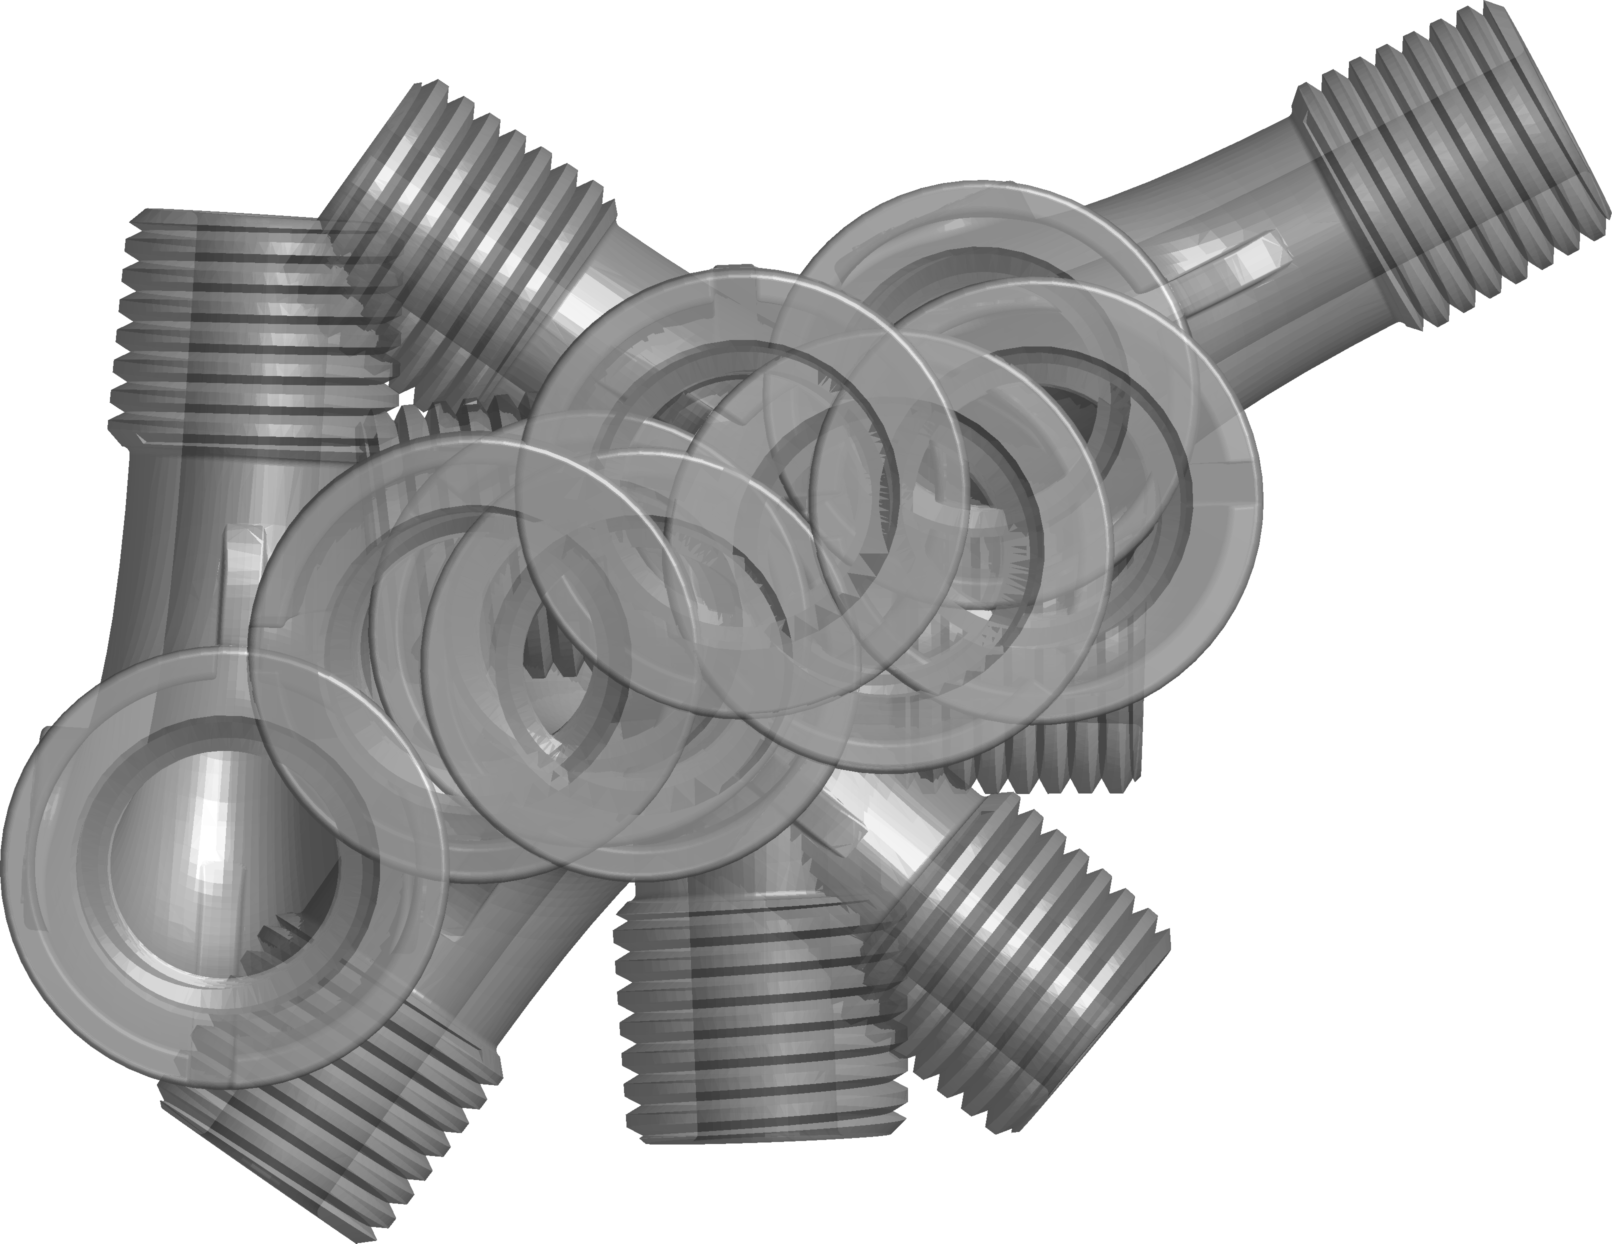
\includegraphics[width=\linewidth]{fig/3dreg/cluster1.png}
		\caption{Scans 1--8}
	\end{subfigure}
	\begin{subfigure}[b]{0.20\linewidth}
		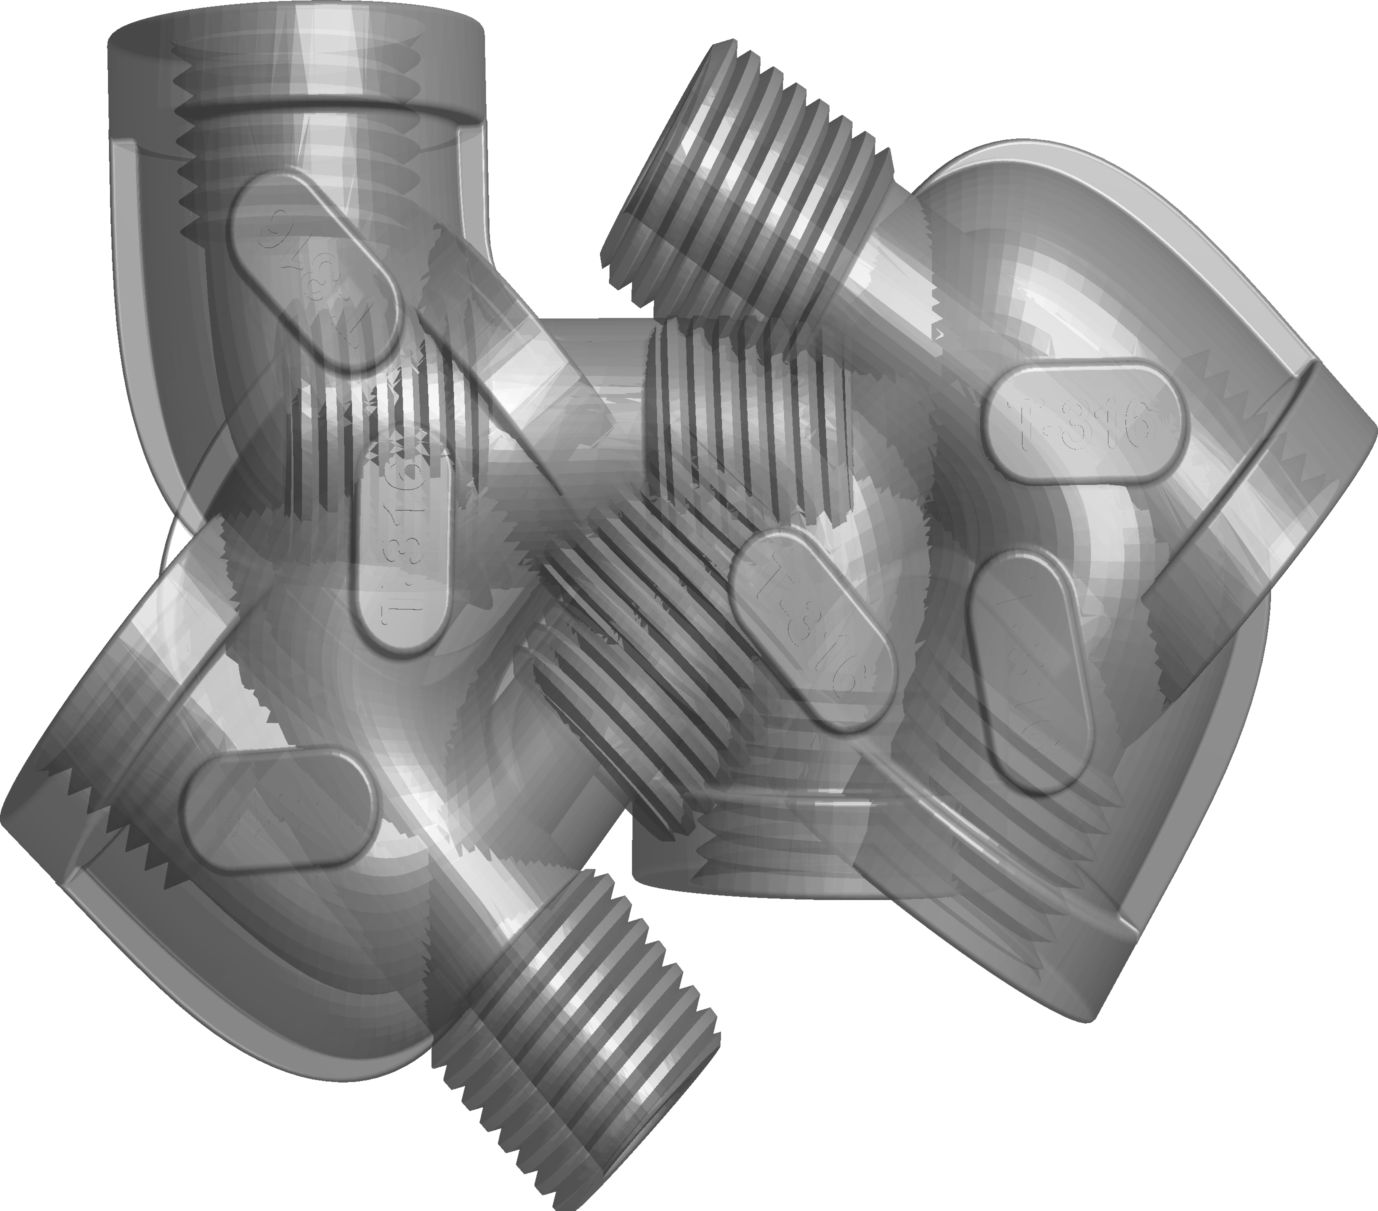
\includegraphics[width=\linewidth]{fig/3dreg/cluster2.png}
		\caption{Scans 9--14}
	\end{subfigure}
	\begin{subfigure}[b]{0.20\linewidth}
		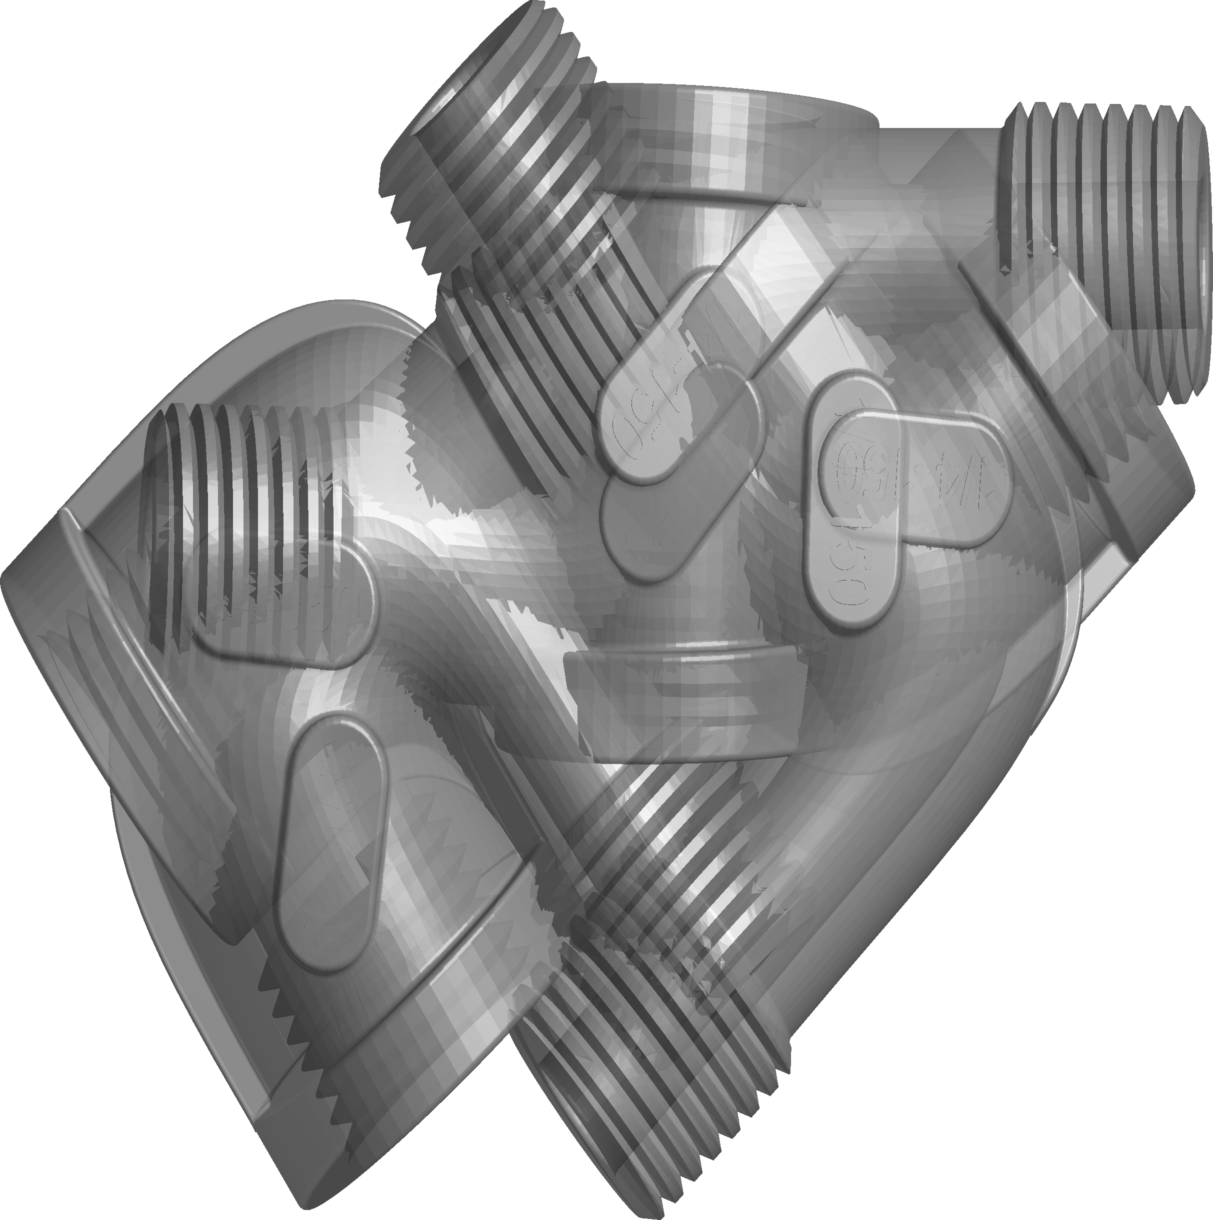
\includegraphics[width=\linewidth]{fig/3dreg/cluster3.png}
		\caption{Scans 15--20}
	\end{subfigure}
	\caption{Raw data captured in three distinct poses for the \emph{pipe} class lead to the three pose clusters shown above.}
	\label{fig:3dclusters}
\end{figure}

%%%%%%%%%%%%%%%%% TRAINING REGISTRATION
\begin{figure}[ht]
\centering
\raisebox{2.5mm}{
\begin{minipage}[!t]{0.24\linewidth}
\centering
\raisebox{1mm}{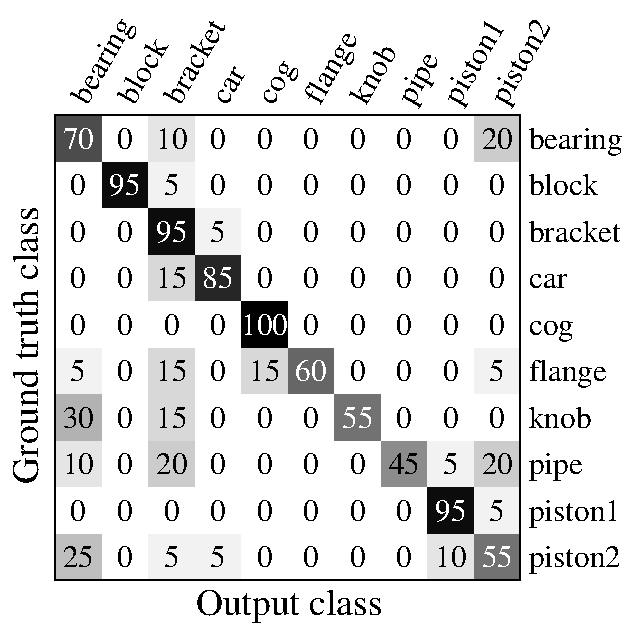
\includegraphics[height=2.5cm]{fig/3dreg/confusion_sap.pdf}}
\caption{Confusion matrix of SAP model.}
\label{fig:confusion_sap}
\end{minipage}
}
\hfill
\vspace{-1mm}
\begin{minipage}[!t]{0.73\linewidth}
\centering
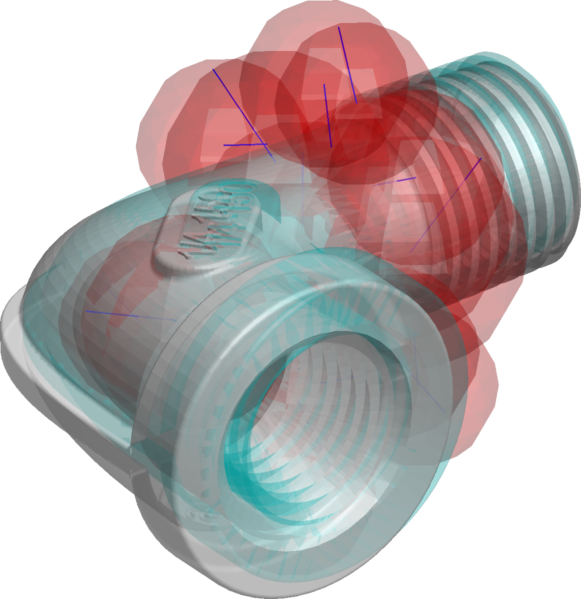
\includegraphics[width=0.098\linewidth]{fig/3dreg/shape01.png} \hspace{-1.5mm}
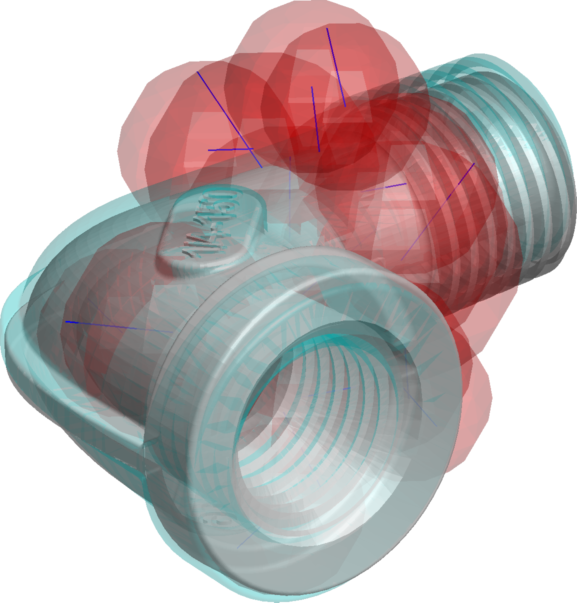
\includegraphics[width=0.098\linewidth]{fig/3dreg/shape02.png} \hspace{-1.5mm}
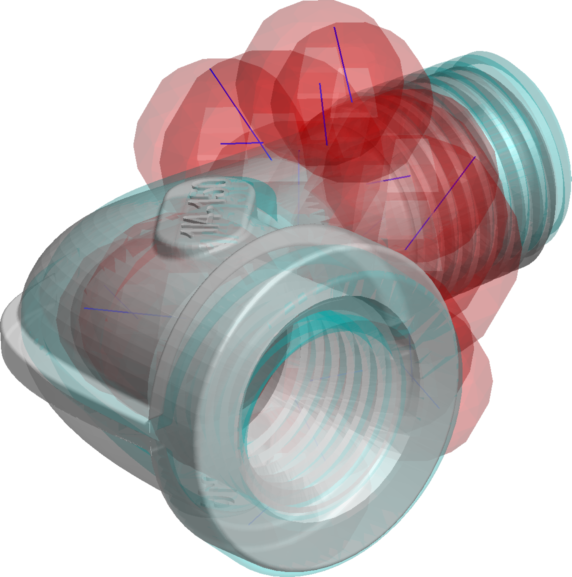
\includegraphics[width=0.098\linewidth]{fig/3dreg/shape03.png} \hspace{-1.5mm}
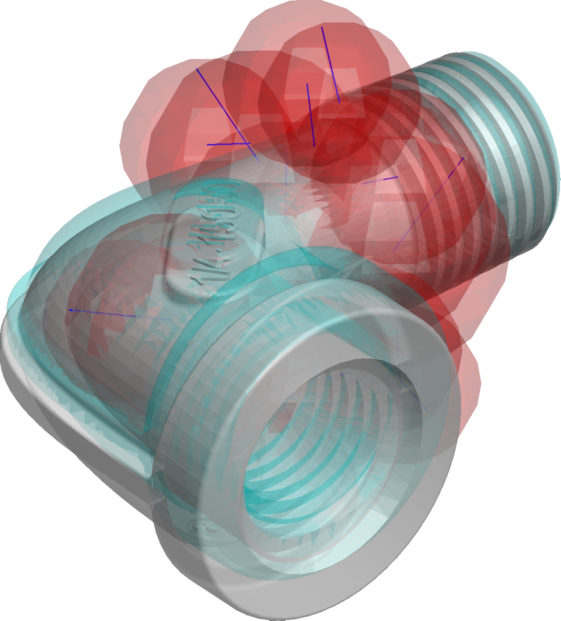
\includegraphics[width=0.098\linewidth]{fig/3dreg/shape04.png} \hspace{-1.5mm}
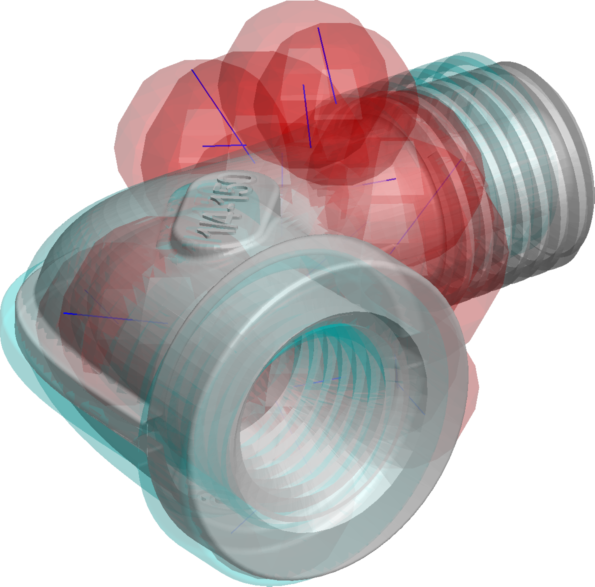
\includegraphics[width=0.098\linewidth]{fig/3dreg/shape05.png} \hspace{-1.5mm}
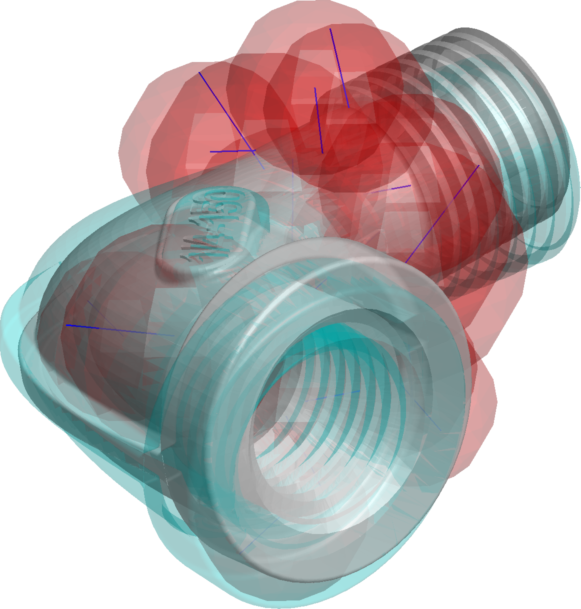
\includegraphics[width=0.098\linewidth]{fig/3dreg/shape06.png} \hspace{-1.5mm}
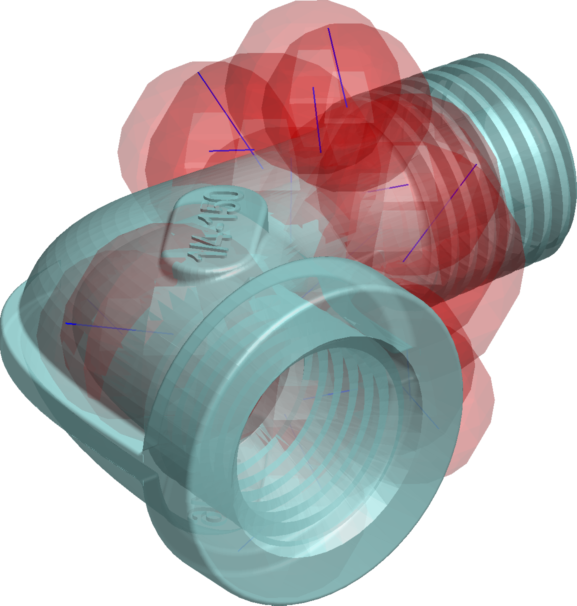
\includegraphics[width=0.098\linewidth]{fig/3dreg/shape07.png} \hspace{-1.5mm}
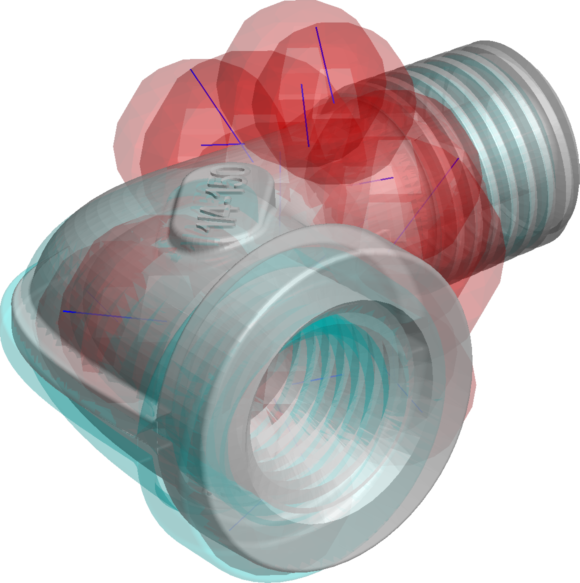
\includegraphics[width=0.098\linewidth]{fig/3dreg/shape08.png} \hspace{-1.5mm} 
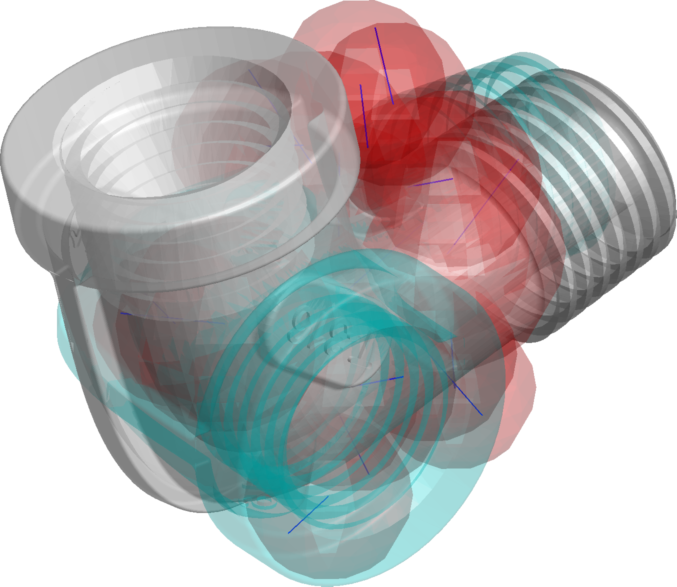
\includegraphics[width=0.098\linewidth]{fig/3dreg/shape09.png} \hspace{-1.5mm}
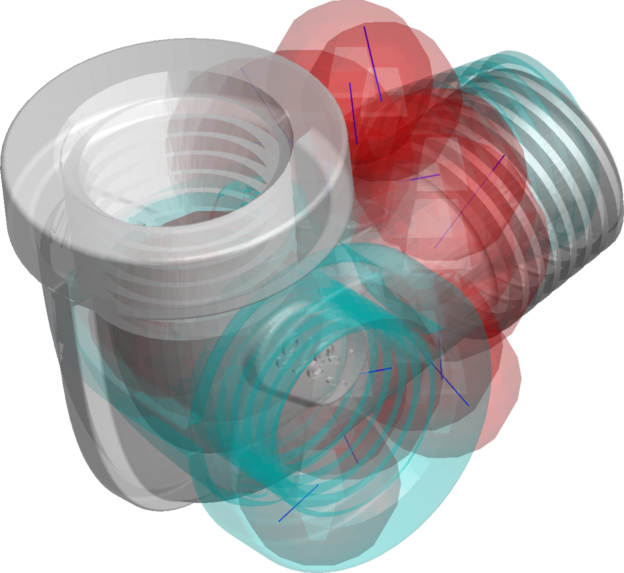
\includegraphics[width=0.098\linewidth]{fig/3dreg/shape10.png} \hspace{-1.5mm} \\ 
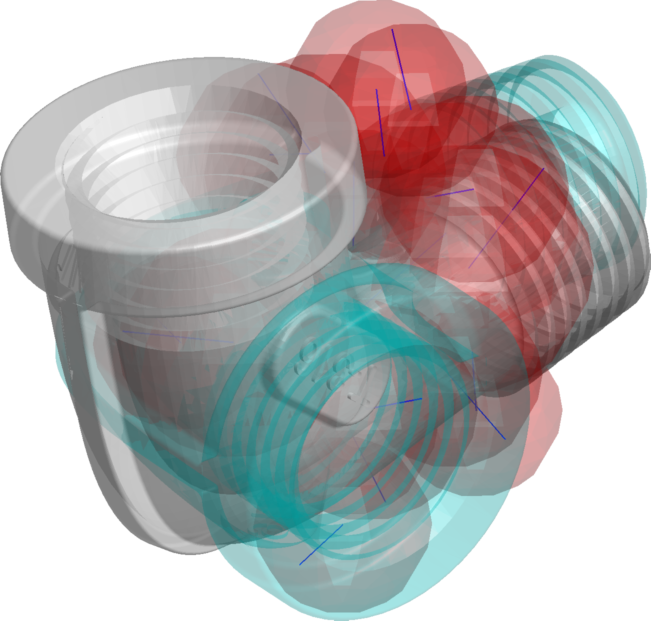
\includegraphics[width=0.098\linewidth]{fig/3dreg/shape11.png} \hspace{-1.5mm}
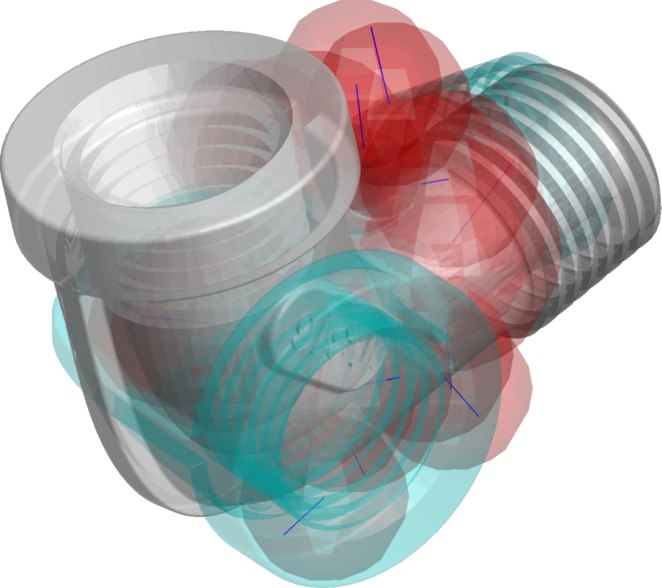
\includegraphics[width=0.098\linewidth]{fig/3dreg/shape12.png} \hspace{-1.5mm}
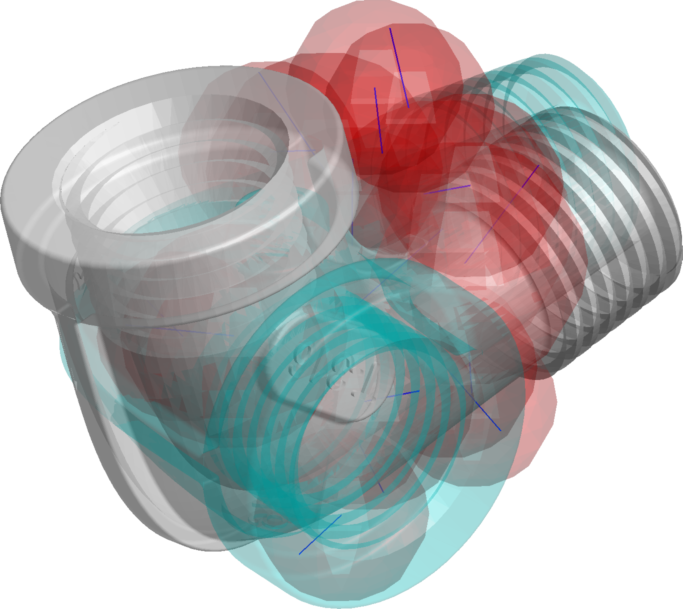
\includegraphics[width=0.098\linewidth]{fig/3dreg/shape13.png} \hspace{-1.5mm}
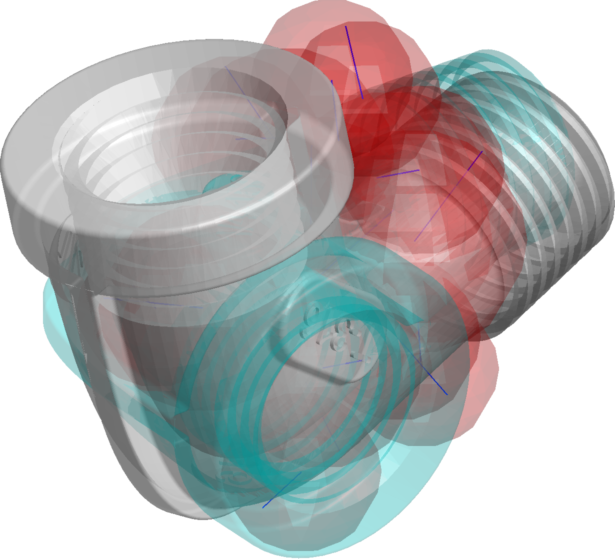
\includegraphics[width=0.098\linewidth]{fig/3dreg/shape14.png} \hspace{-1.5mm} 
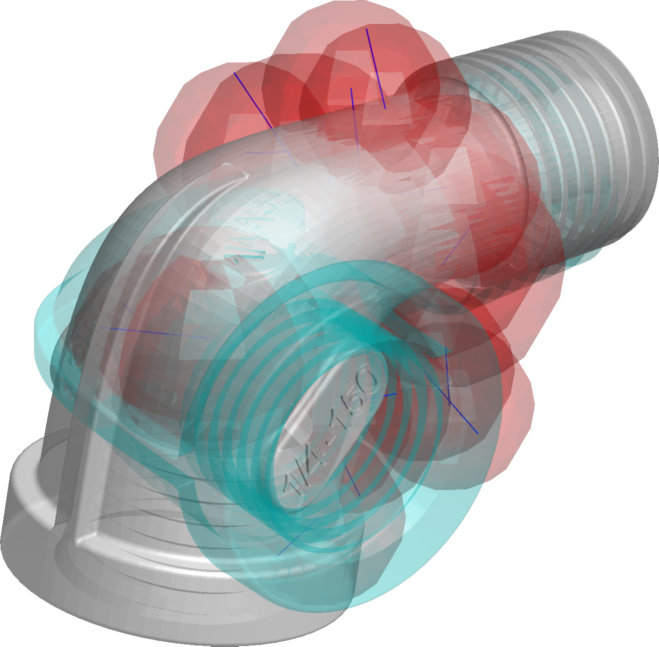
\includegraphics[width=0.098\linewidth]{fig/3dreg/shape15.png} \hspace{-1.5mm}
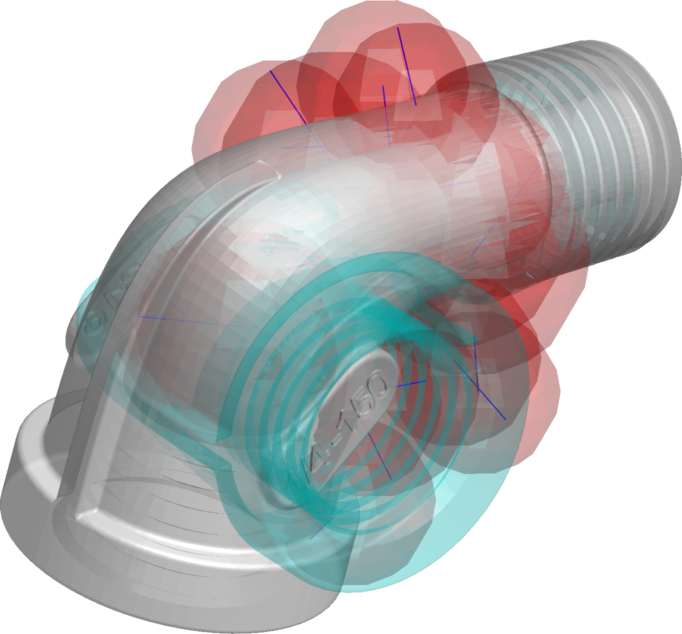
\includegraphics[width=0.098\linewidth]{fig/3dreg/shape16.png} \hspace{-1.5mm}
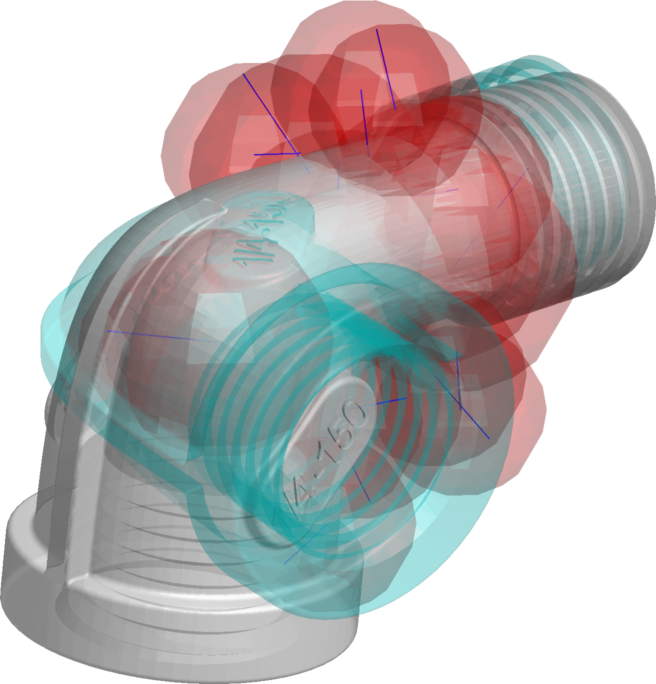
\includegraphics[width=0.098\linewidth]{fig/3dreg/shape17.png} \hspace{-1.5mm}
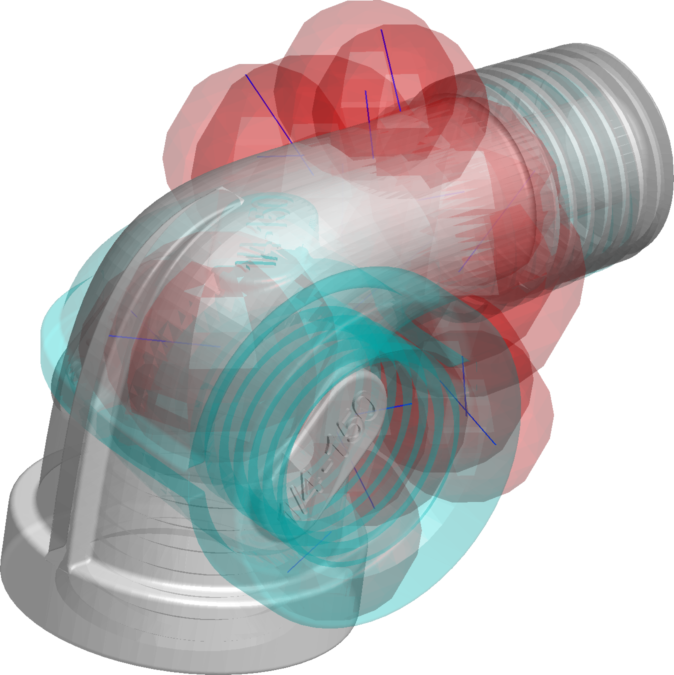
\includegraphics[width=0.098\linewidth]{fig/3dreg/shape18.png} \hspace{-1.5mm}
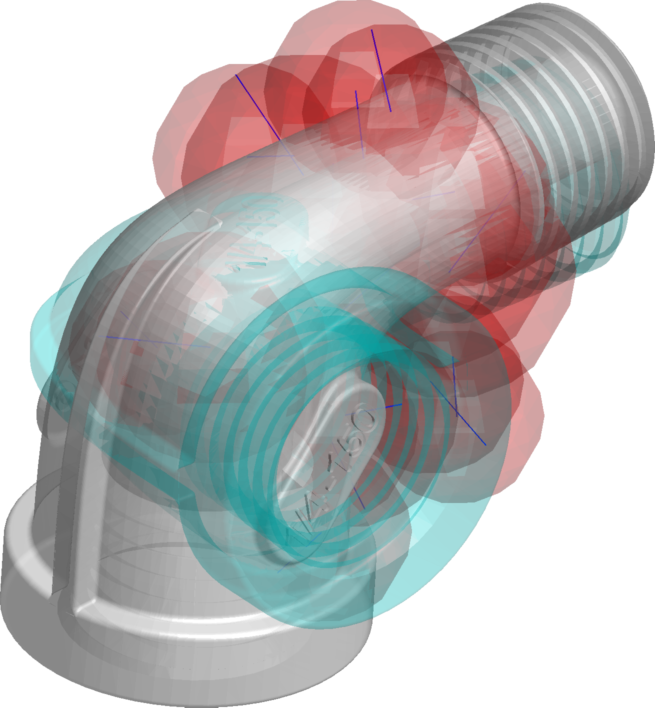
\includegraphics[width=0.098\linewidth]{fig/3dreg/shape19.png} \hspace{-1.5mm}
\includegraphics[width=0.098\linewidth]{fig/3dreg/shape20.png} \vspace{2mm}
\caption{\emph{Grey}: Inferred poses of the 20 \emph{pipe} class training instances. \emph{Cyan}: The \emph{canonical pose}. \emph{Red}: The locations and scales of parts.}
\label{fig:alignresult3d}
\end{minipage}
\end{figure}

For evaluation of registration in training, every training instance is compared with each of the 20 instances, giving a $20\!\times\!20$ SRT distance matrix. Figure \ref{fig:3dreg_srtmatrices} visualizes these matrices for several classes in the \emph{Point Cloud} dataset, demonstrating that for some classes, distinct pose clusters form. Figure \ref{fig:alignresult3d} indicates that these clusters form around a small number of distinct poses that the object was captured in, possibly latching onto background features in this situation also. Figure \ref{fig:3dclusters} visualizes the groups of distinct poses of the point clouds, showing that the clustering issue is originated from the raw data captured. Initializing poses to the groundtruth during learning still leads to these clusters. Since the \emph{Bike} dataset consists of images of different bikes on different backgrounds, it does not suffer from this issue.

%%%%%%%%%%%%%%%%% TESTING REGISTRATION
In test, we use the evaluation framework of \cite{Pham2011}; the $\tilde{\pose}$ of each test instance is compared to that of the training instance which gives the lowest Euclidean distance of its part-wise likelihood with that of the test instance. The per-class registration results are given in table \ref{tab:regresult3d}, where they are compared with state-of-the-art results of a supervised (\ie groundtruth poses used in training), vote-based approach \cite{Woodford2013}. Despite the SAP model having the handicap of not using groundtruth pose, it obtains the highest score on half the classes.

\begin{table}[t]
\centering
{\footnotesize
\begin{tabular}{|c|c|c|c|c|c|c|c|c|c|c|c|c|}
\hline
\multirow{2}{*}{\textbf{Method}} & \multicolumn{10}{|c|}{\textbf{Category}} & \multirow{2}{*}{\textbf{Average}} \\
\cline{2-11}
& \rotatebox{90}{{bearing}}& 
\rotatebox{90}{{block}}& 
\rotatebox{90}{{bracket}}& 
\rotatebox{90}{{car}}& 
\rotatebox{90}{{cog}}& 
\rotatebox{90}{{flange}}& 
\rotatebox{90}{{knob}}& 
\rotatebox{90}{{pipe}}& 
\rotatebox{90}{{piston1}} & 
\rotatebox{90}{{piston2}} & \\
\hline
SAP ($\numpart = 15, \numparticle = 10$)%\remarka
 & 50 & \textbf{35} & \textbf{100} & 75 & \textbf{100} & \textbf{60} & 65 & 25 & 45 & \textbf{95} & 65.0\\
\hline
Min.-ent. H.~\cite{Woodford2013}\remarkb 			& \textbf{83} & 20 & 98 & \textbf{91} & \textbf{100} & 36 & \textbf{91} & \textbf{89} & \textbf{54} & 84 & \textbf{74.6}\\
\hline
\end{tabular}
\vspace{2mm}
}
\caption{Object registration results for the \emph{Point Cloud} dataset. {\footnotesize \remarkb Trained using groundtruth poses.}}
\label{tab:regresult3d}
\end{table}

\section{Conclusions}
\label{sec:conclusions}
% recap of our work
We have presented a generative shape, appearance and pose (SAP) model and inference framework, which jointly learns a constellation model and the poses of training instances, additionally providing registration capability on top of recognition. In doing so we have solved the difficult optimization problem created by a vastly increased parameter space, by introducing a novel, particle-based optimization scheme.

% experiments
We have demonstrated not only that inferring pose jointly with shape and appearance is feasible in practice, but that in doing so, our method performs only marginally worse than methods which use groundtruth pose, and significantly improves on other approaches when groundtruth pose is not known.

% what is so important? and future work?
We hope that this work will lead to object recognition systems learned from large-scale, un-annotated datasets, including those which use only the estimated registrations from training to then learn a different type of model. We plan to extend this approach to learn a 3D constellation model of an object, along with 3D poses, from a series of 2D images.
